% Created 2023-08-04 Fri 12:24
% Intended LaTeX compiler: pdflatex
\documentclass[11pt]{article}
\usepackage[utf8]{inputenc}
\usepackage[T1]{fontenc}
\usepackage{graphicx}
\usepackage{longtable}
\usepackage{wrapfig}
\usepackage{rotating}
\usepackage[normalem]{ulem}
\usepackage{amsmath}
\usepackage{amssymb}
\usepackage{capt-of}
\usepackage{hyperref}
\usepackage{kotex}
\author{holy}
\date{\textit{<2023-08-03 Thu>}}
\title{[sql] programmers sql high score2}
\hypersetup{
 pdfauthor={holy},
 pdftitle={[sql] programmers sql high score2},
 pdfkeywords={},
 pdfsubject={programmers 문제 풀이},
 pdfcreator={Emacs 30.0.50 (Org mode 9.6.6)}, 
 pdflang={English}}
\begin{document}

\maketitle
\tableofcontents



\section*{problem1: 강원도에 위치한 생상공장 목록 출력하기(level1)}
\label{sec:org4b278c7}
\begin{center}
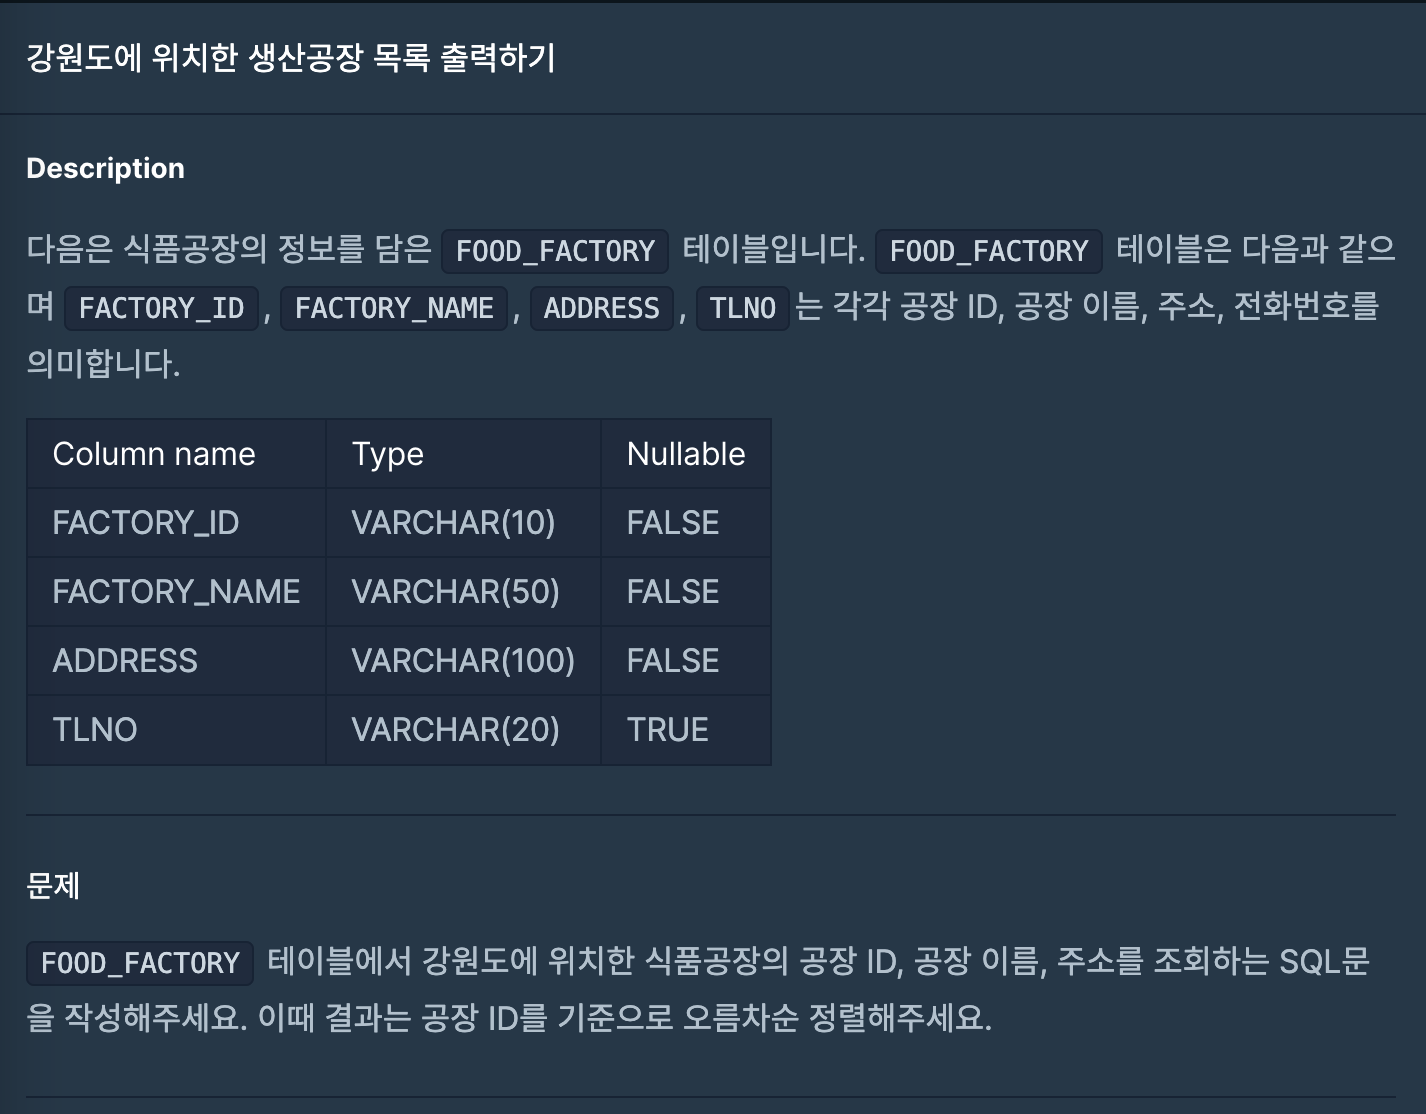
\includegraphics[width=400px]{../static/img/sql/p1-1.png}
\end{center}
\begin{center}
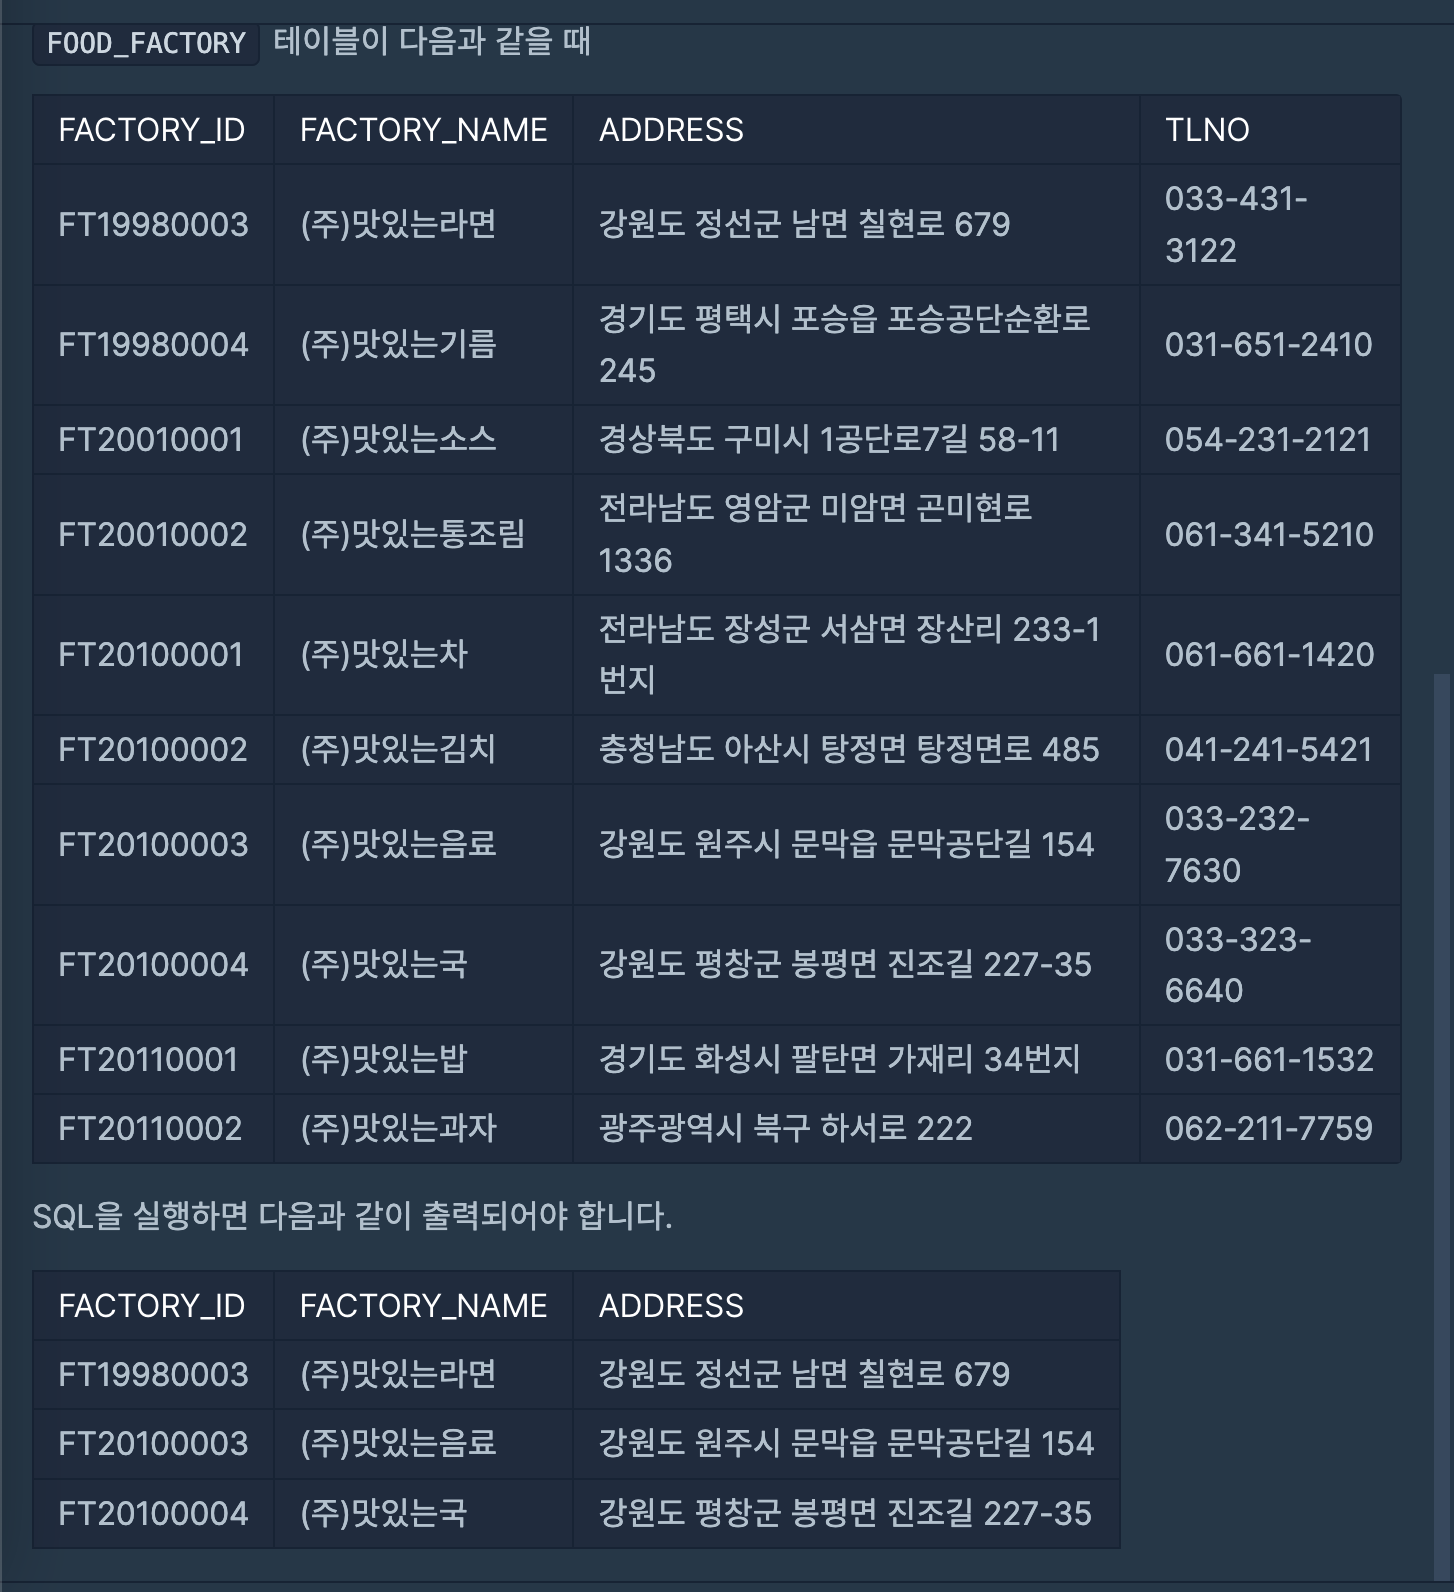
\includegraphics[width=400px]{../static/img/sql/p1-2.png}
\end{center}
\section*{풀이}
\label{sec:org4b03bce}
푸는 순서는 다음과 같다. from부터 푼다. 이문제에서 어려울것은 없다. 
\subsection*{from FOOD\_FACTORY}
\label{sec:org2bafc1d}
\subsection*{select FACTORY\_ID, FACTORY\_NAME,ADDRESS from FOOD\_Factory}
\label{sec:org9201c04}
\subsection*{select FACTORY\_ID, FACTORY\_NAME,ADDRESS from FOOD\_Factory order by FACTORY\_ID asc}
\label{sec:org88363c1}

\section*{problem2: 흉부외과 또는 일반 외과 의사 목록 출력하기(level1)}
\label{sec:org832083b}
\begin{center}
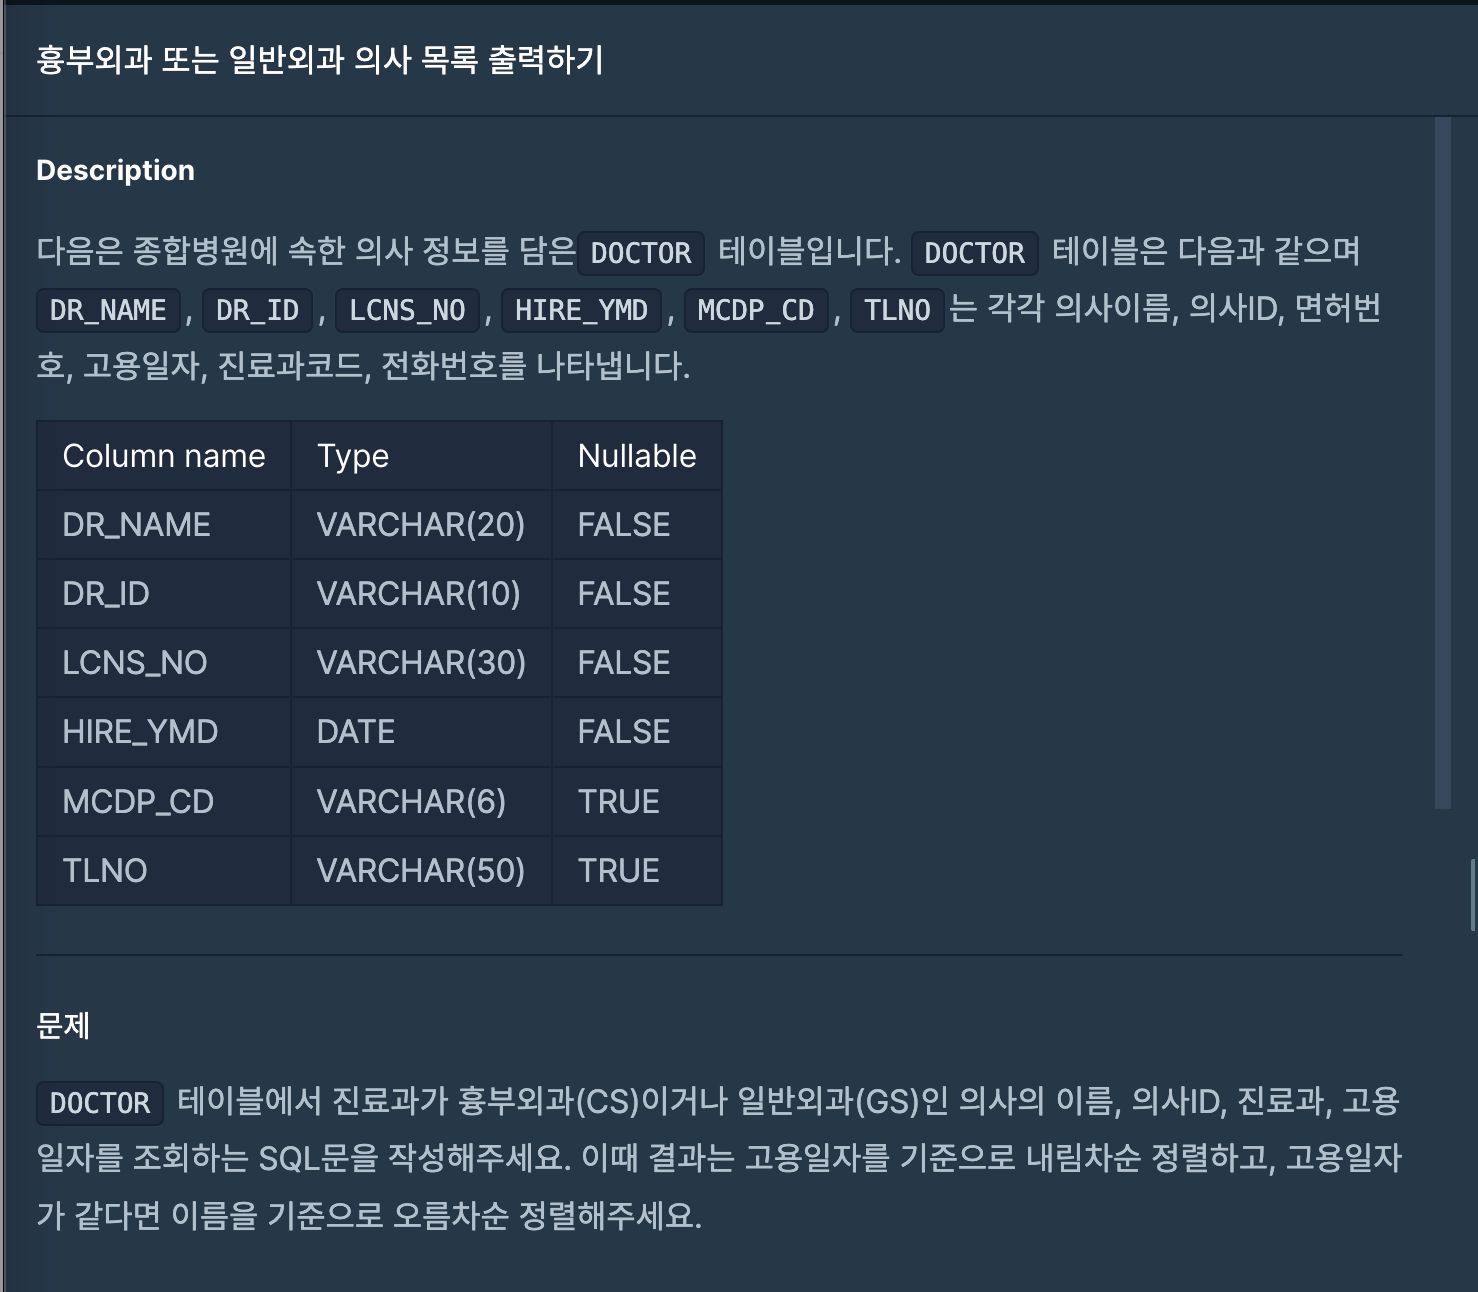
\includegraphics[width=100px]{../static/img/sql/p2-1.png}
\end{center}
\begin{center}
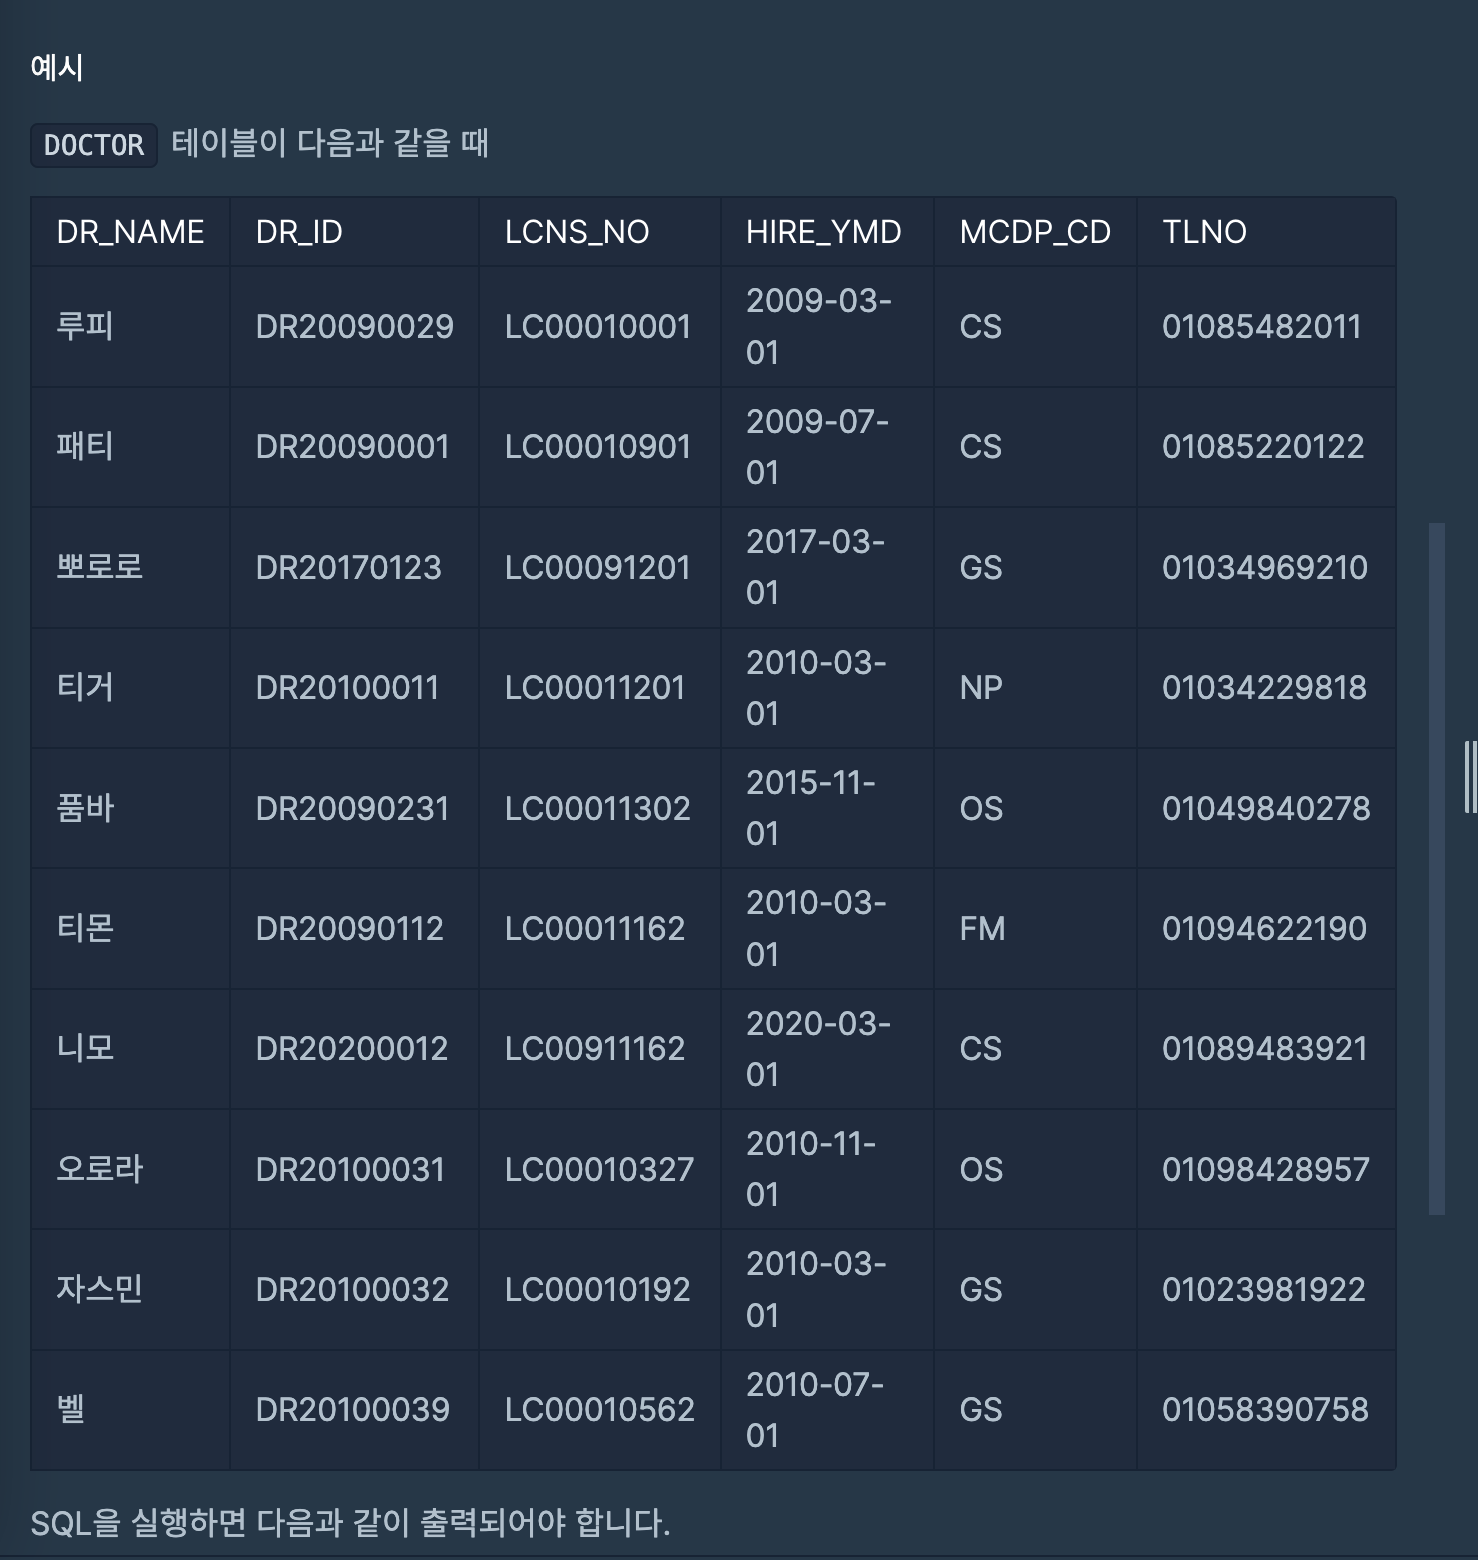
\includegraphics[width=100px]{../static/img/sql/p2-2.png}
\end{center}
\begin{center}
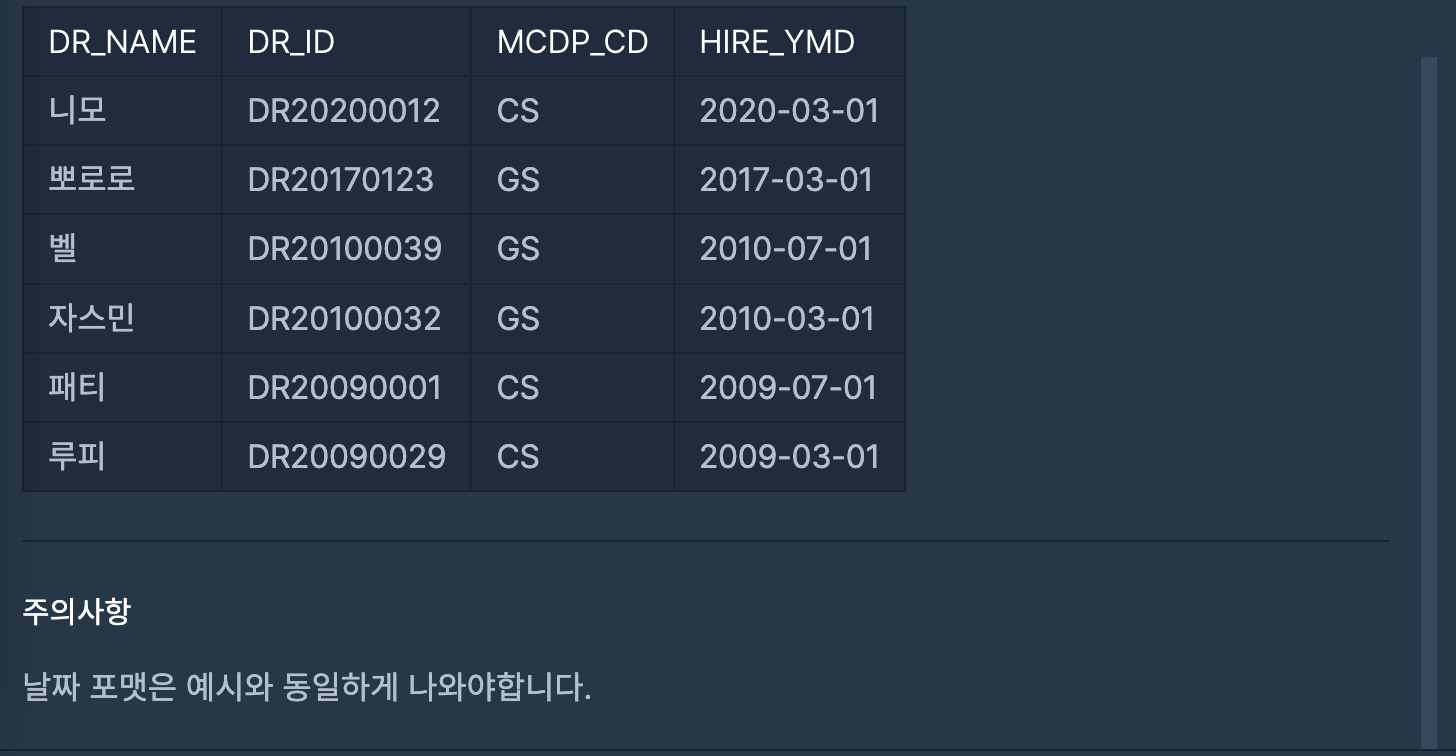
\includegraphics[width=100px]{../static/img/sql/p2-3.png}
\end{center}

\section*{풀이}
\label{sec:org26428a9}

\section*{problem3: 서울에 위치한 식당 목록 출력하기(level4)}
\label{sec:org62d8c8d}
\begin{center}
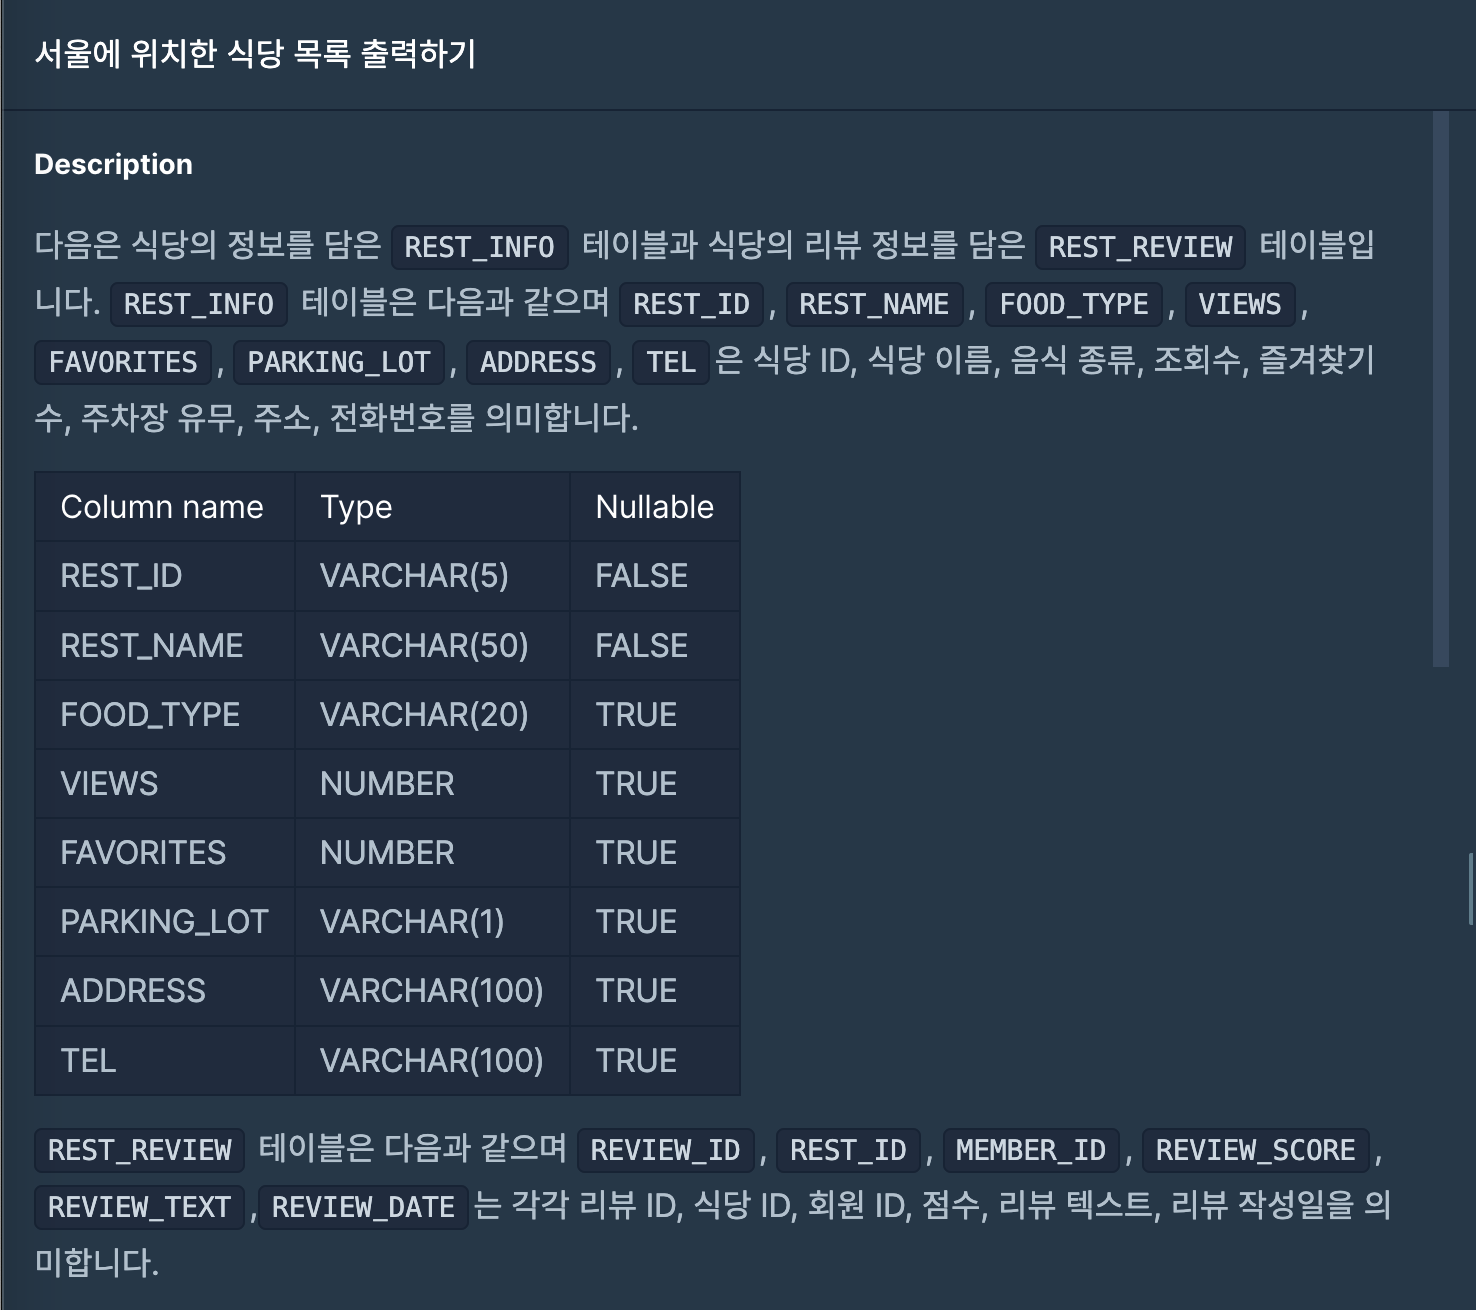
\includegraphics[width=100px]{../static/img/sql/p3-1.png}
\end{center}
\begin{center}
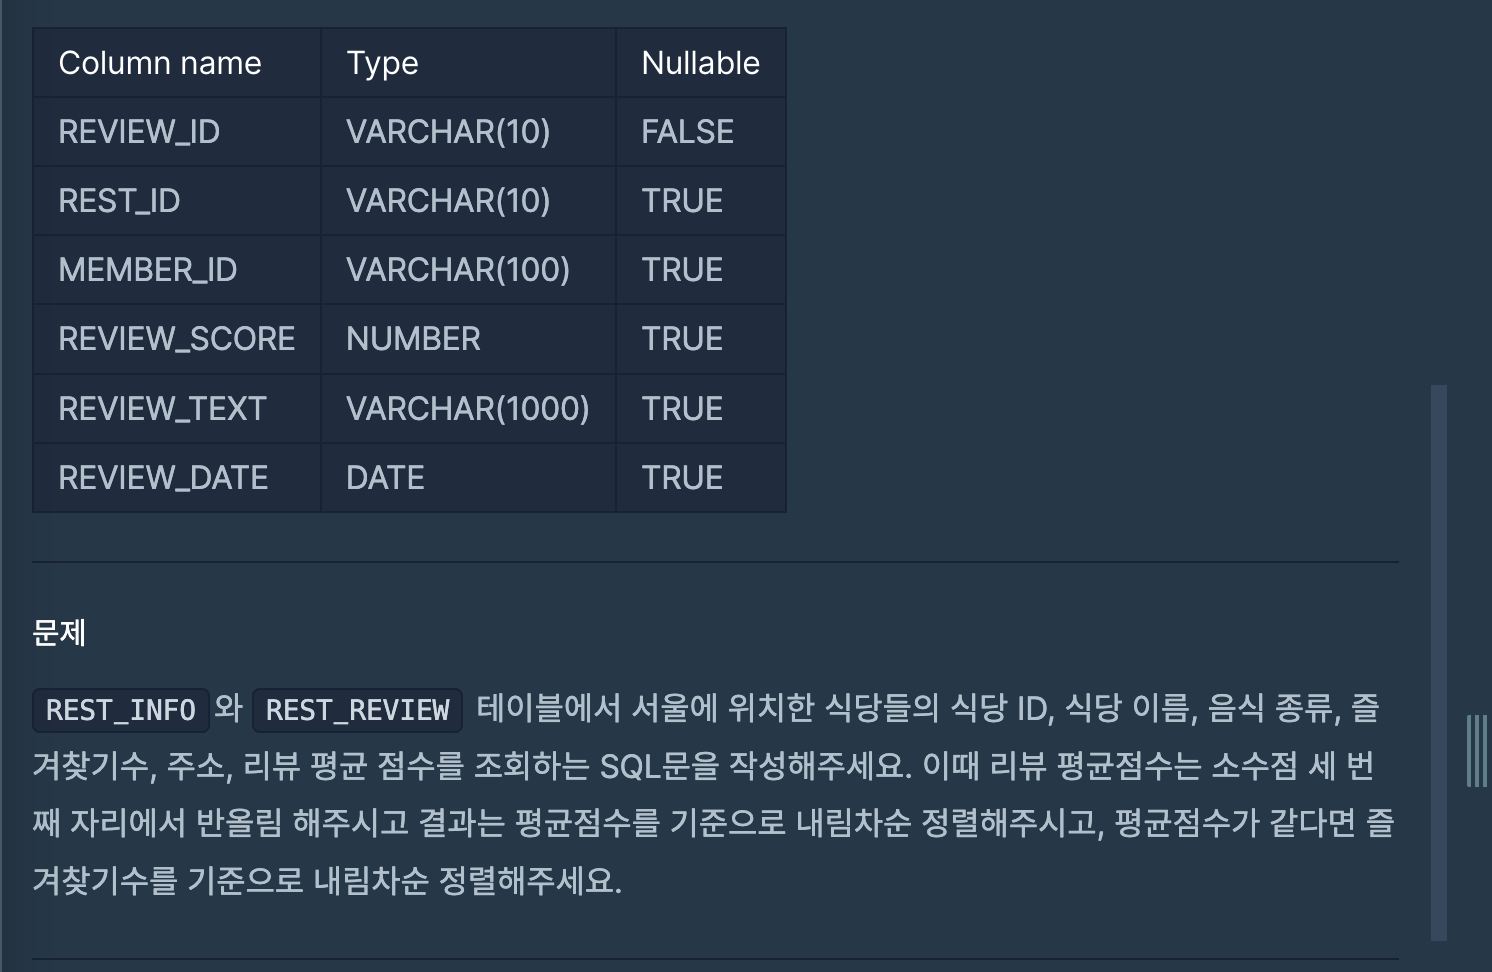
\includegraphics[width=100px]{../static/img/sql/p3-2.png}
\end{center}
\begin{center}
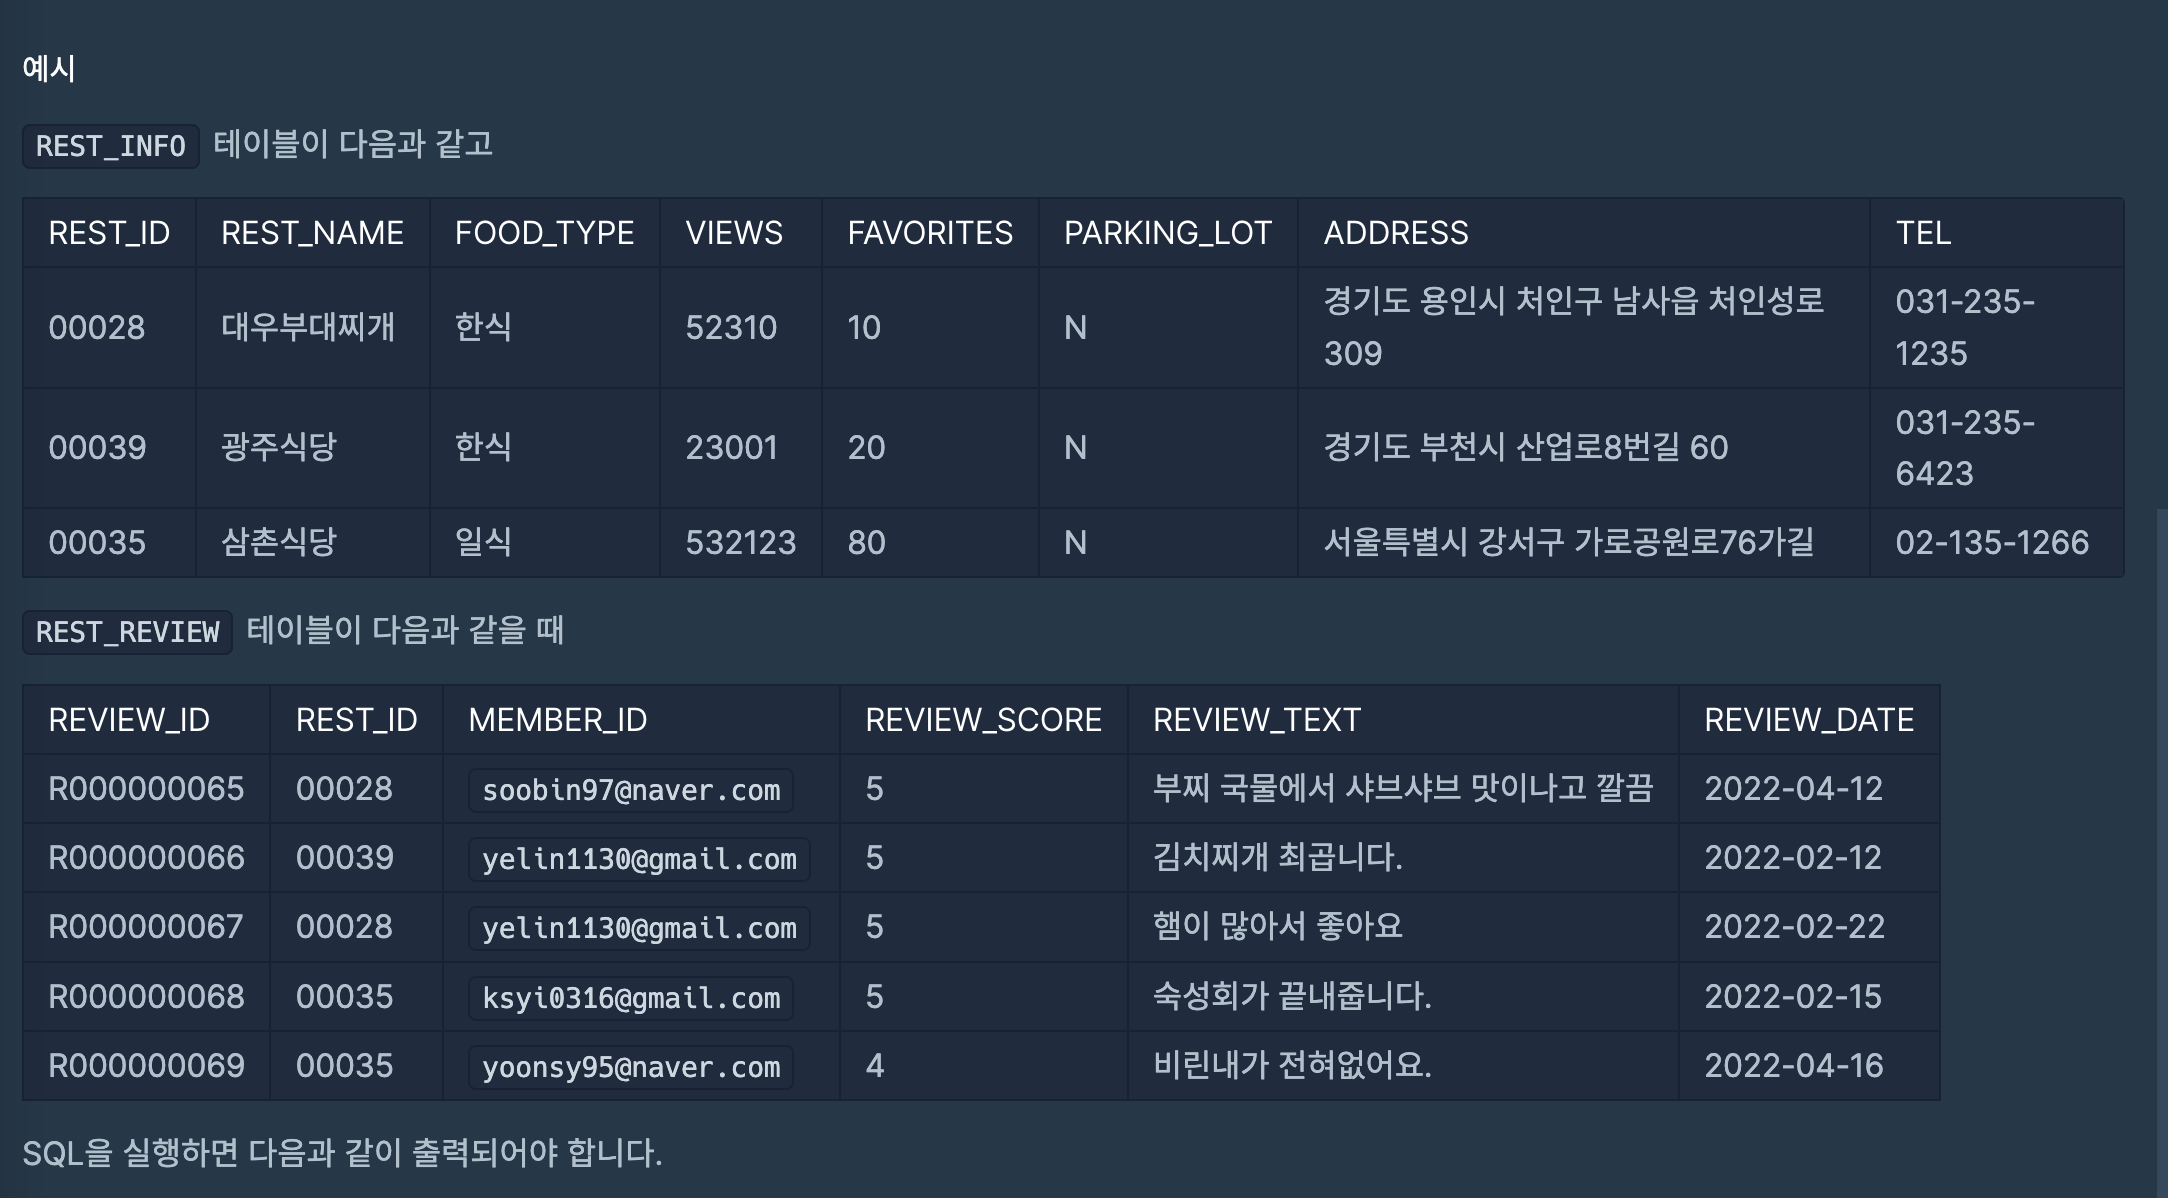
\includegraphics[width=100px]{../static/img/sql/p3-3.png}
\end{center}
\begin{center}
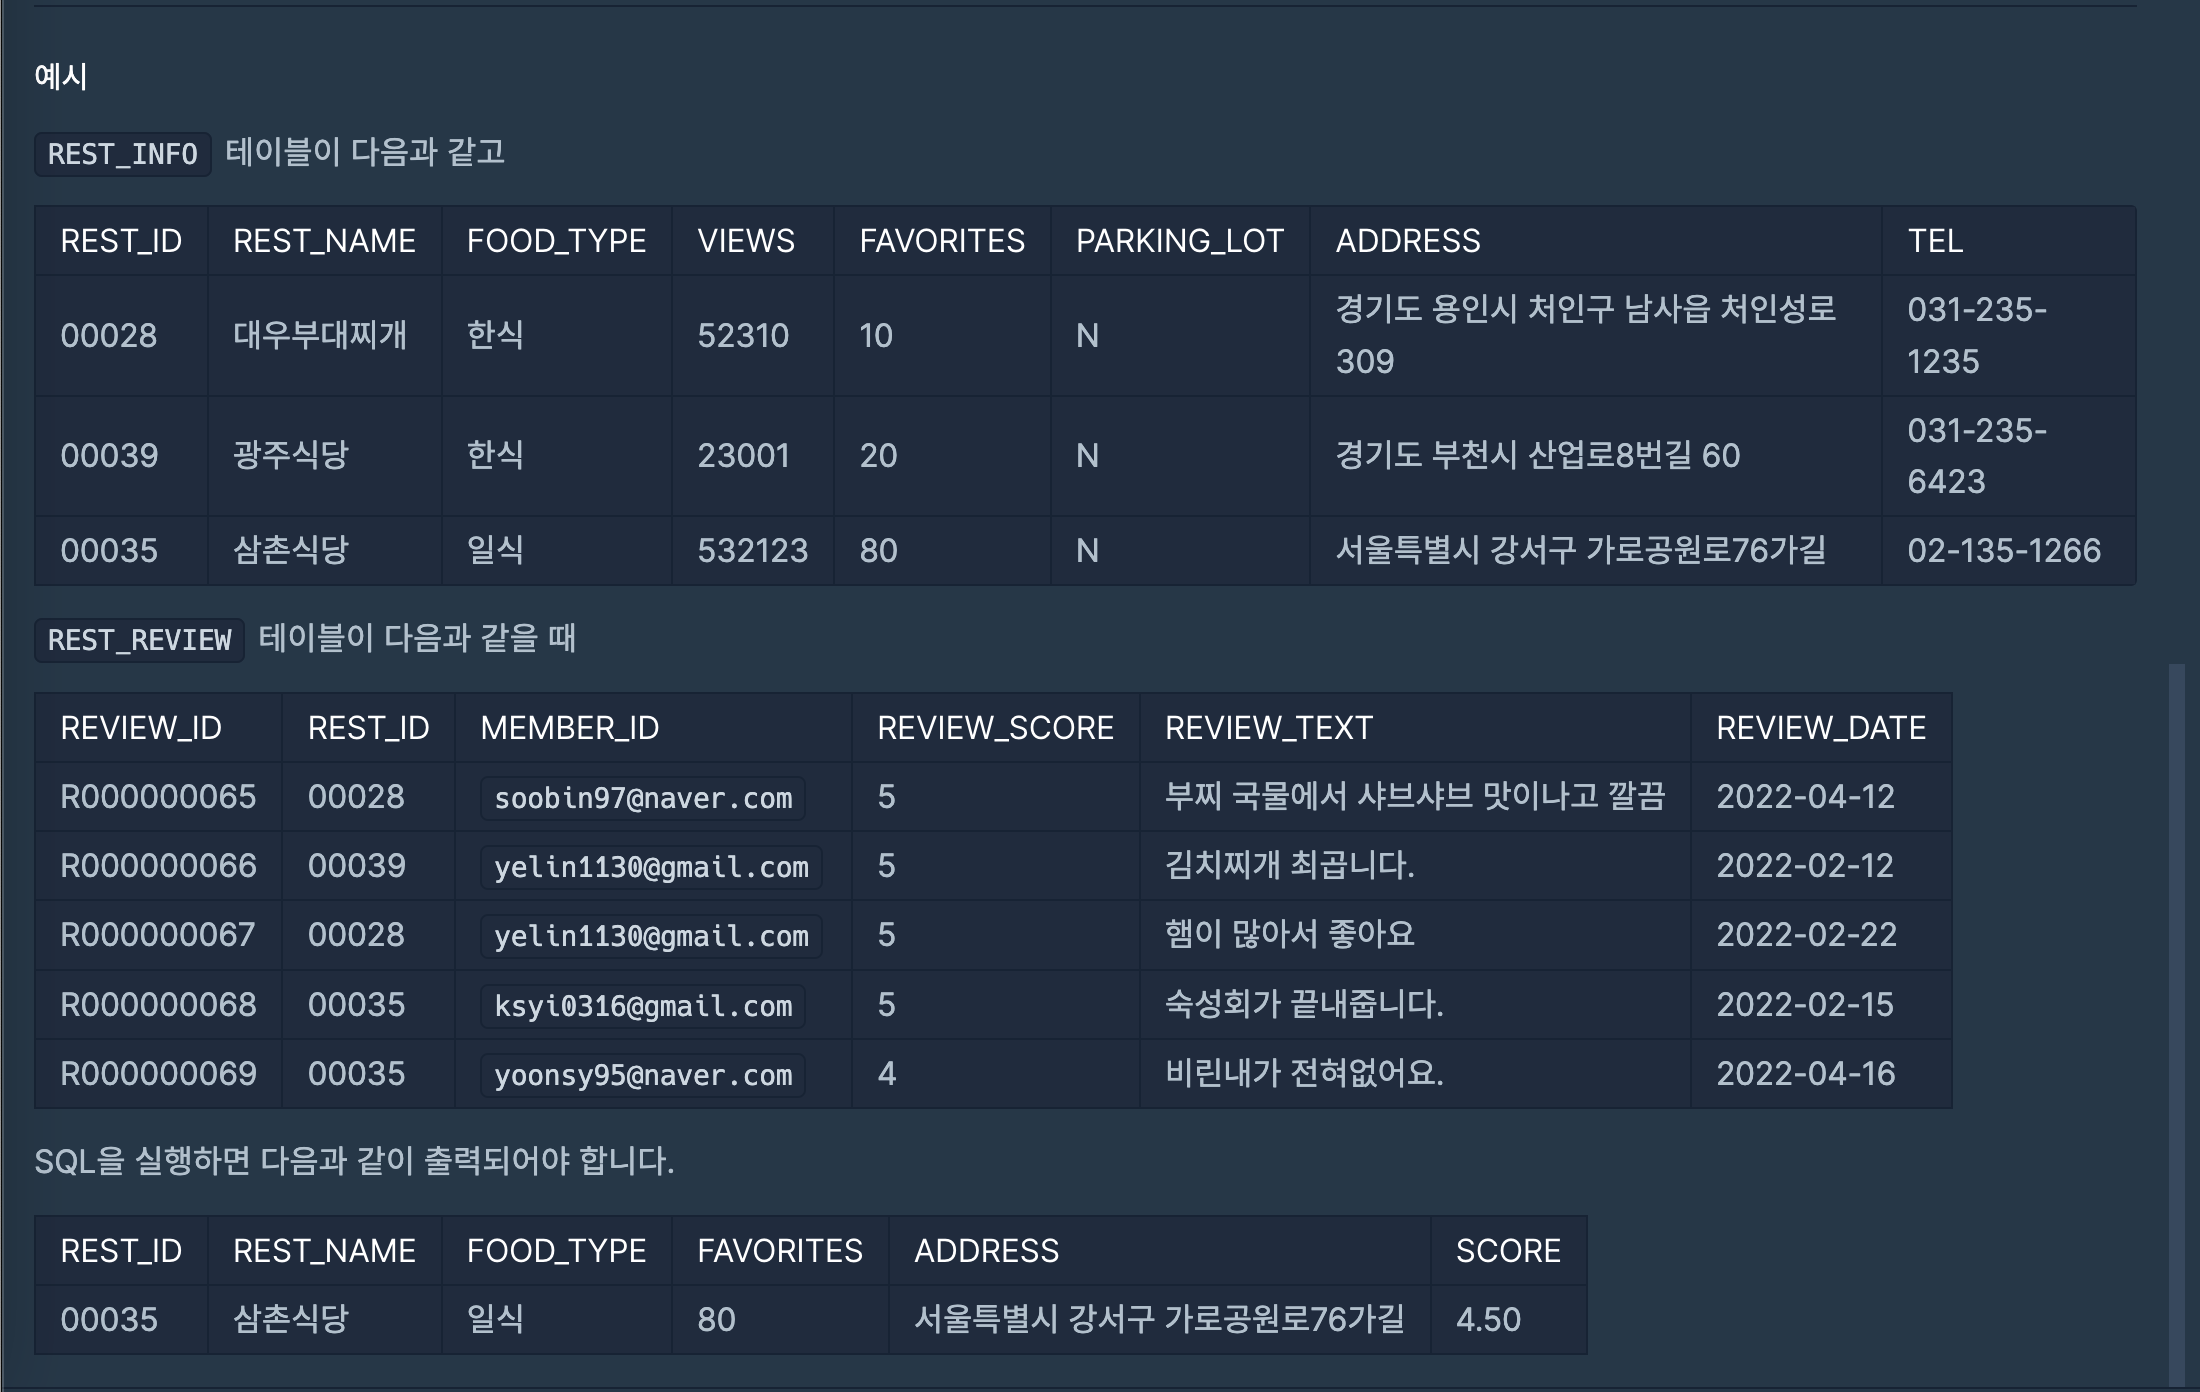
\includegraphics[width=100px]{../static/img/sql/p3-4.png}
\end{center}

\section*{풀이}
\label{sec:orgeaefb0b}

\section*{problem4: 조건에 맞는 도서 리스트 출력하기(level1)}
\label{sec:orgd387b19}
\begin{center}
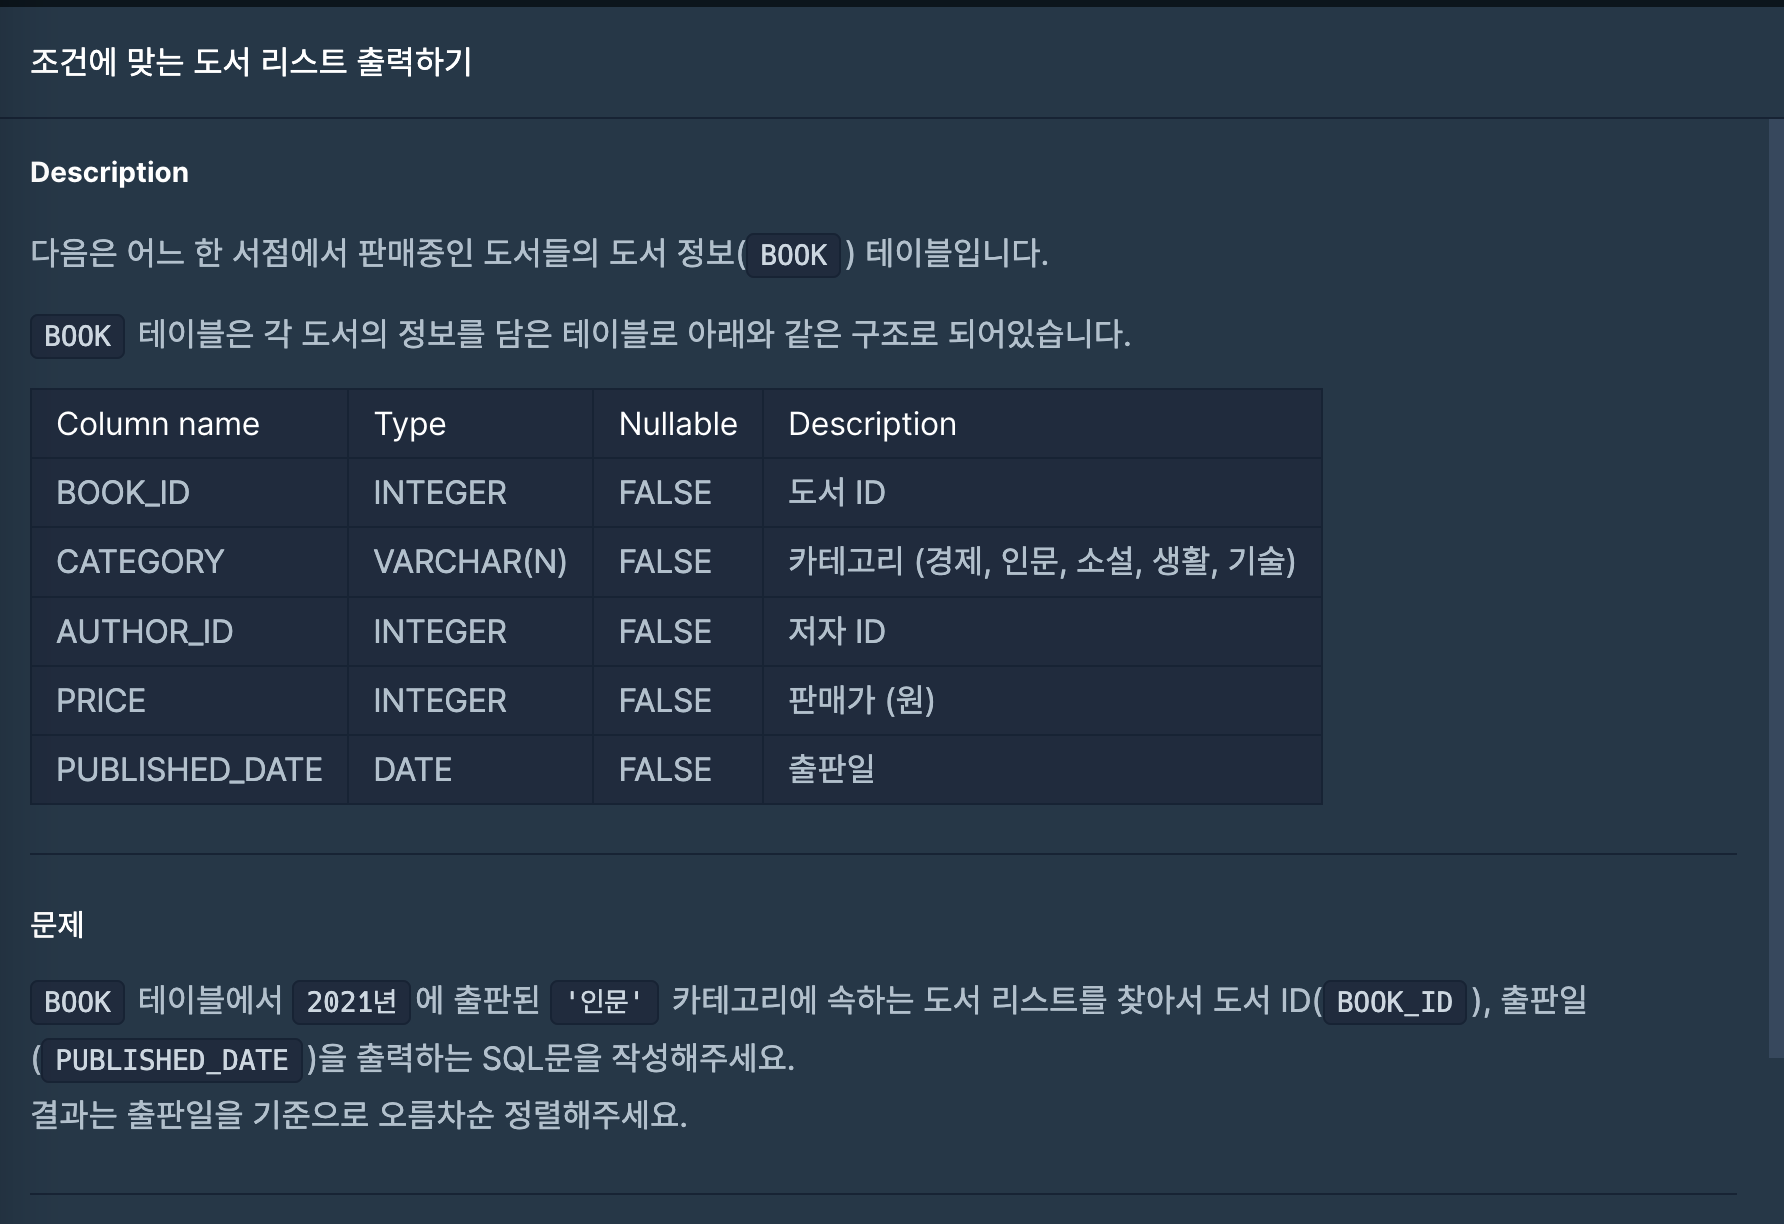
\includegraphics[width=100px]{../static/img/sql/p4-1.png}
\end{center}
\begin{center}
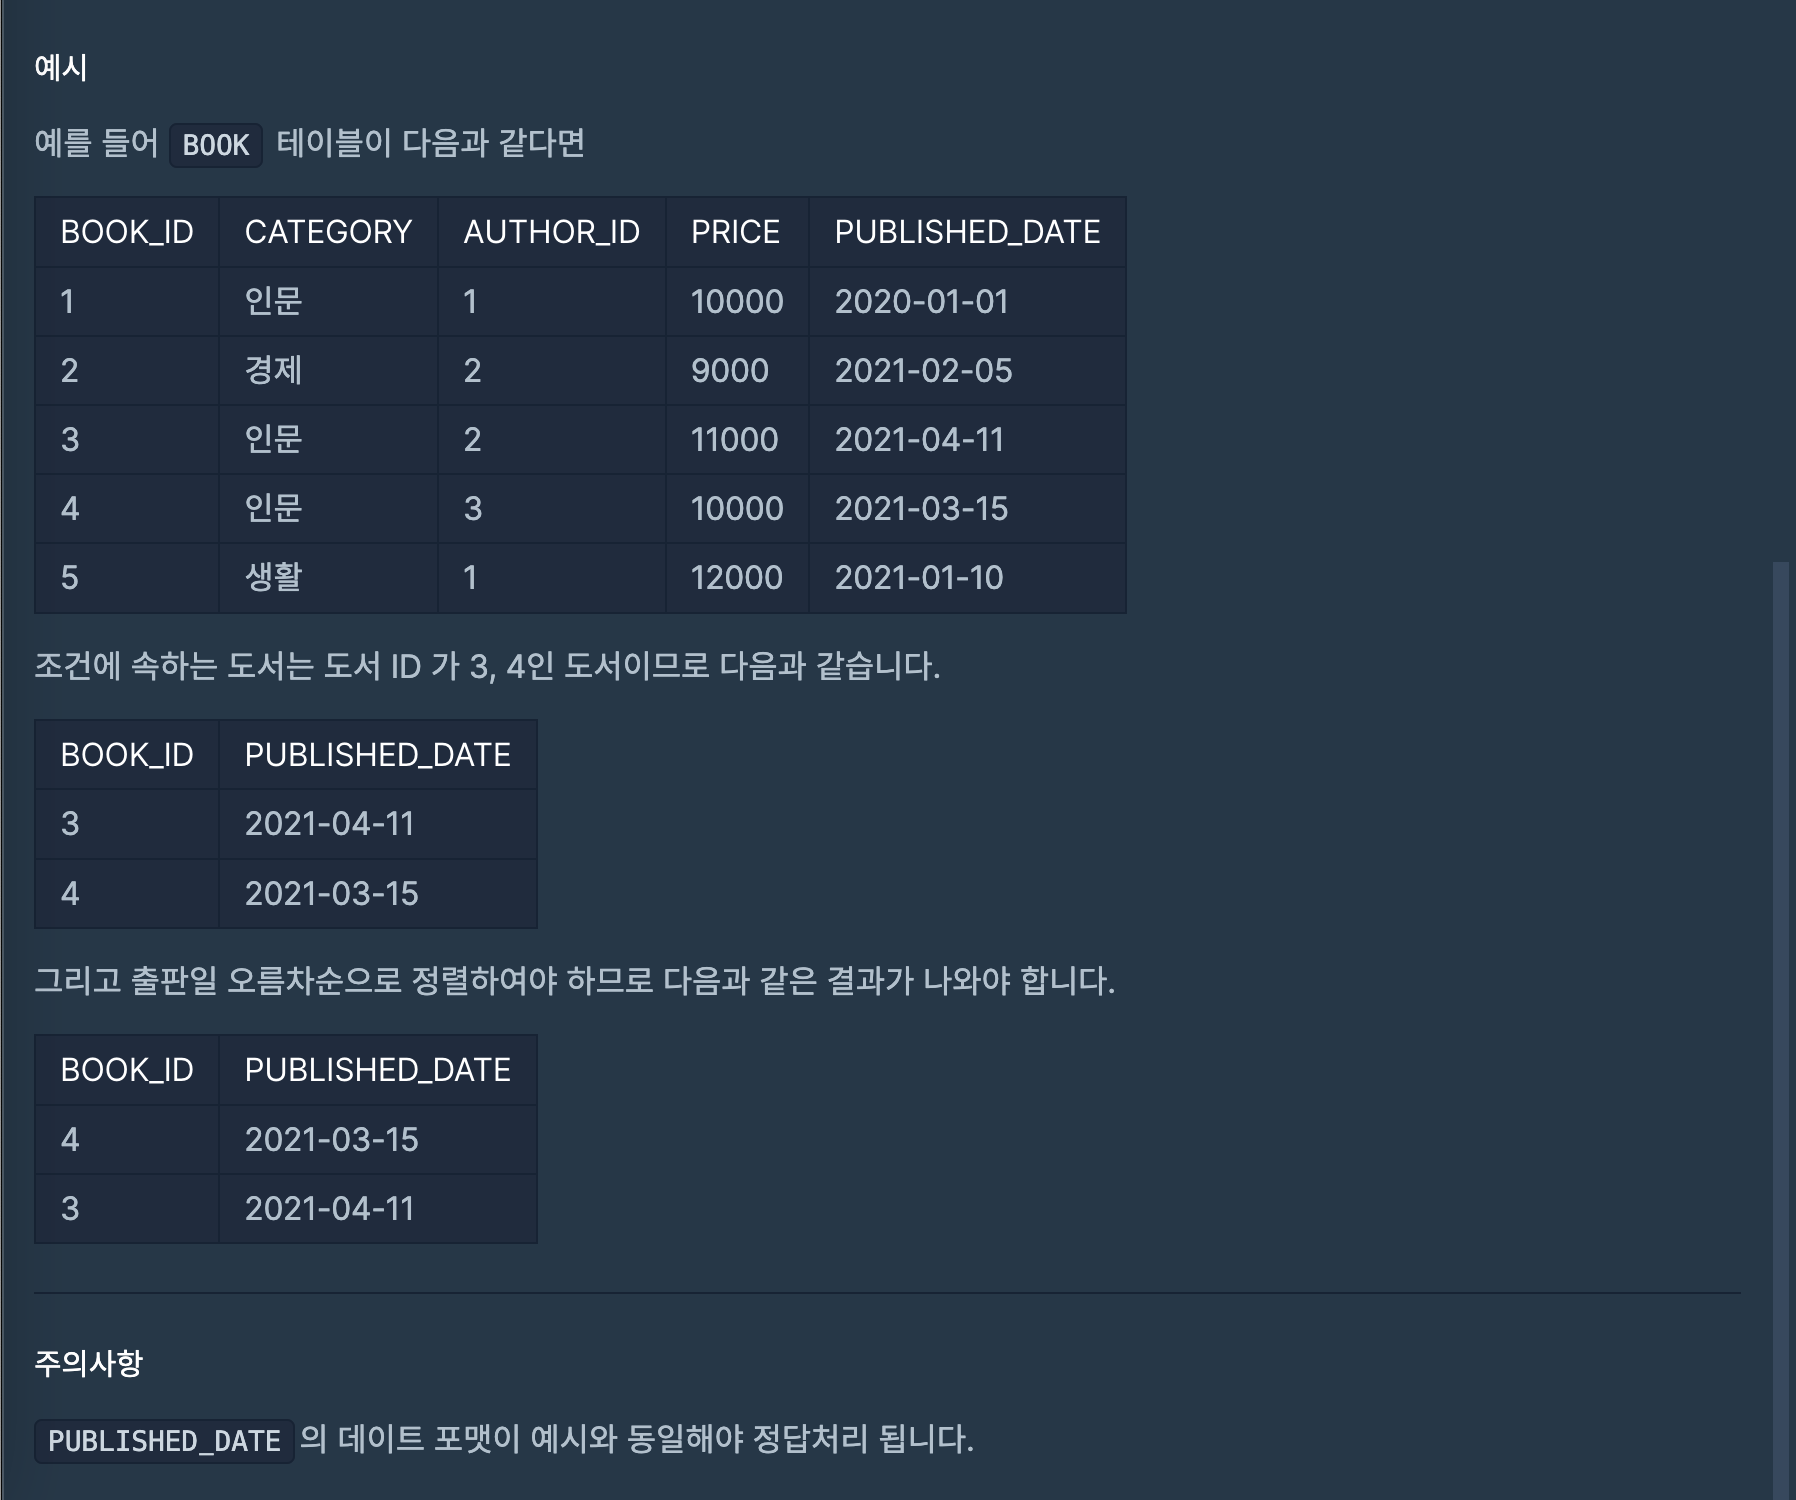
\includegraphics[width=100px]{../static/img/sql/p4-2.png}
\end{center}

\section*{풀이}
\label{sec:org79852a1}

\section*{problem5: 과일로 만든 아이스크림 고르기(level1)}
\label{sec:orgd4b263c}
\begin{center}
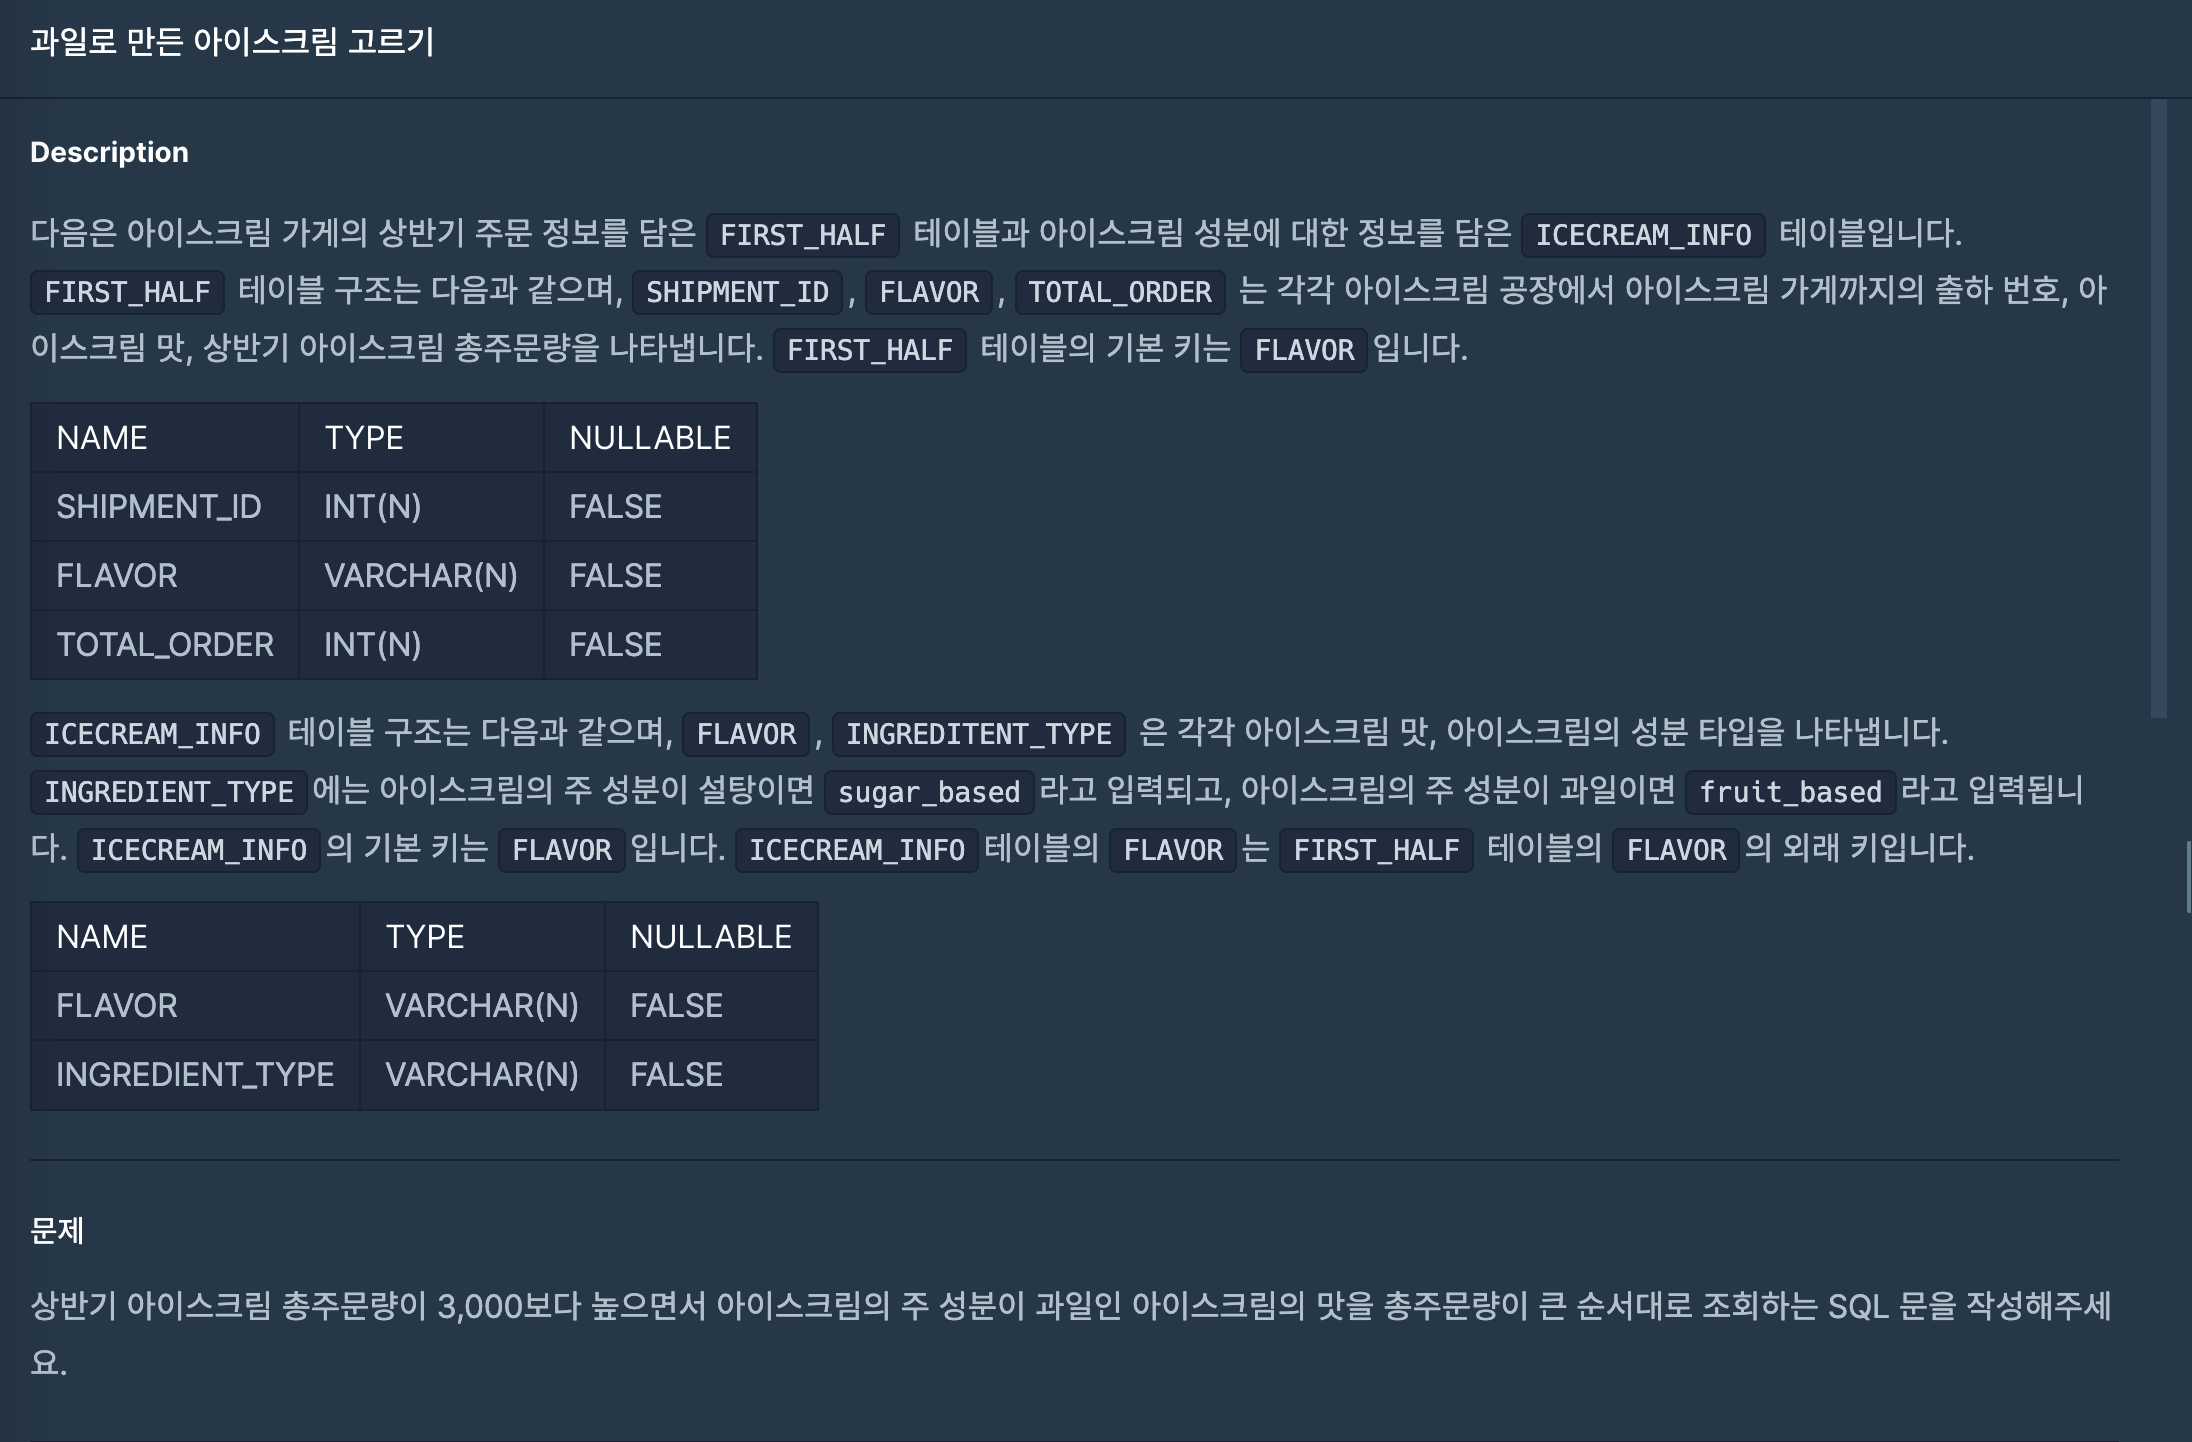
\includegraphics[width=100px]{../static/img/sql/p5-1.png}
\end{center}

\begin{center}
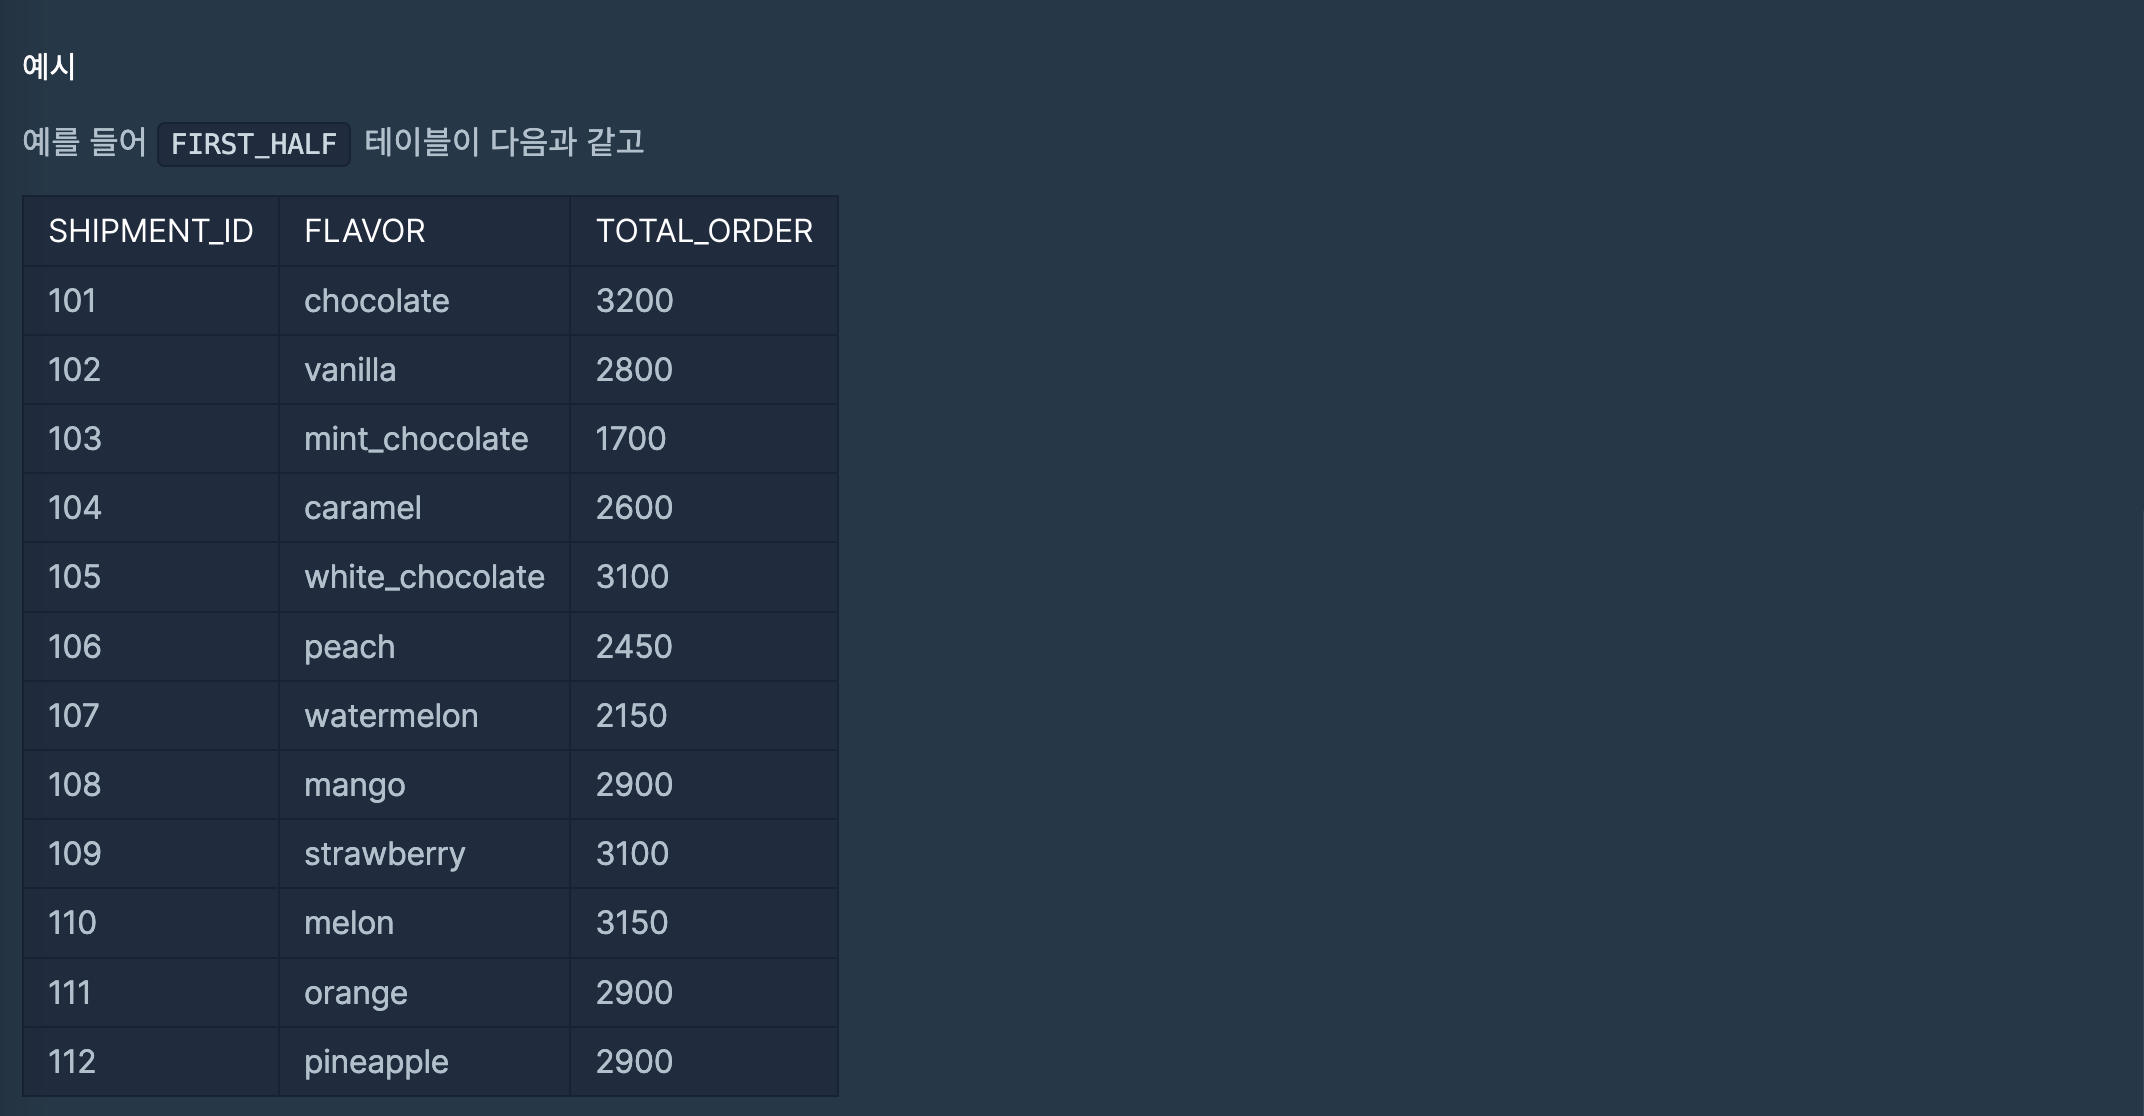
\includegraphics[width=100px]{../static/img/sql/p5-2.png}
\end{center}

\begin{center}
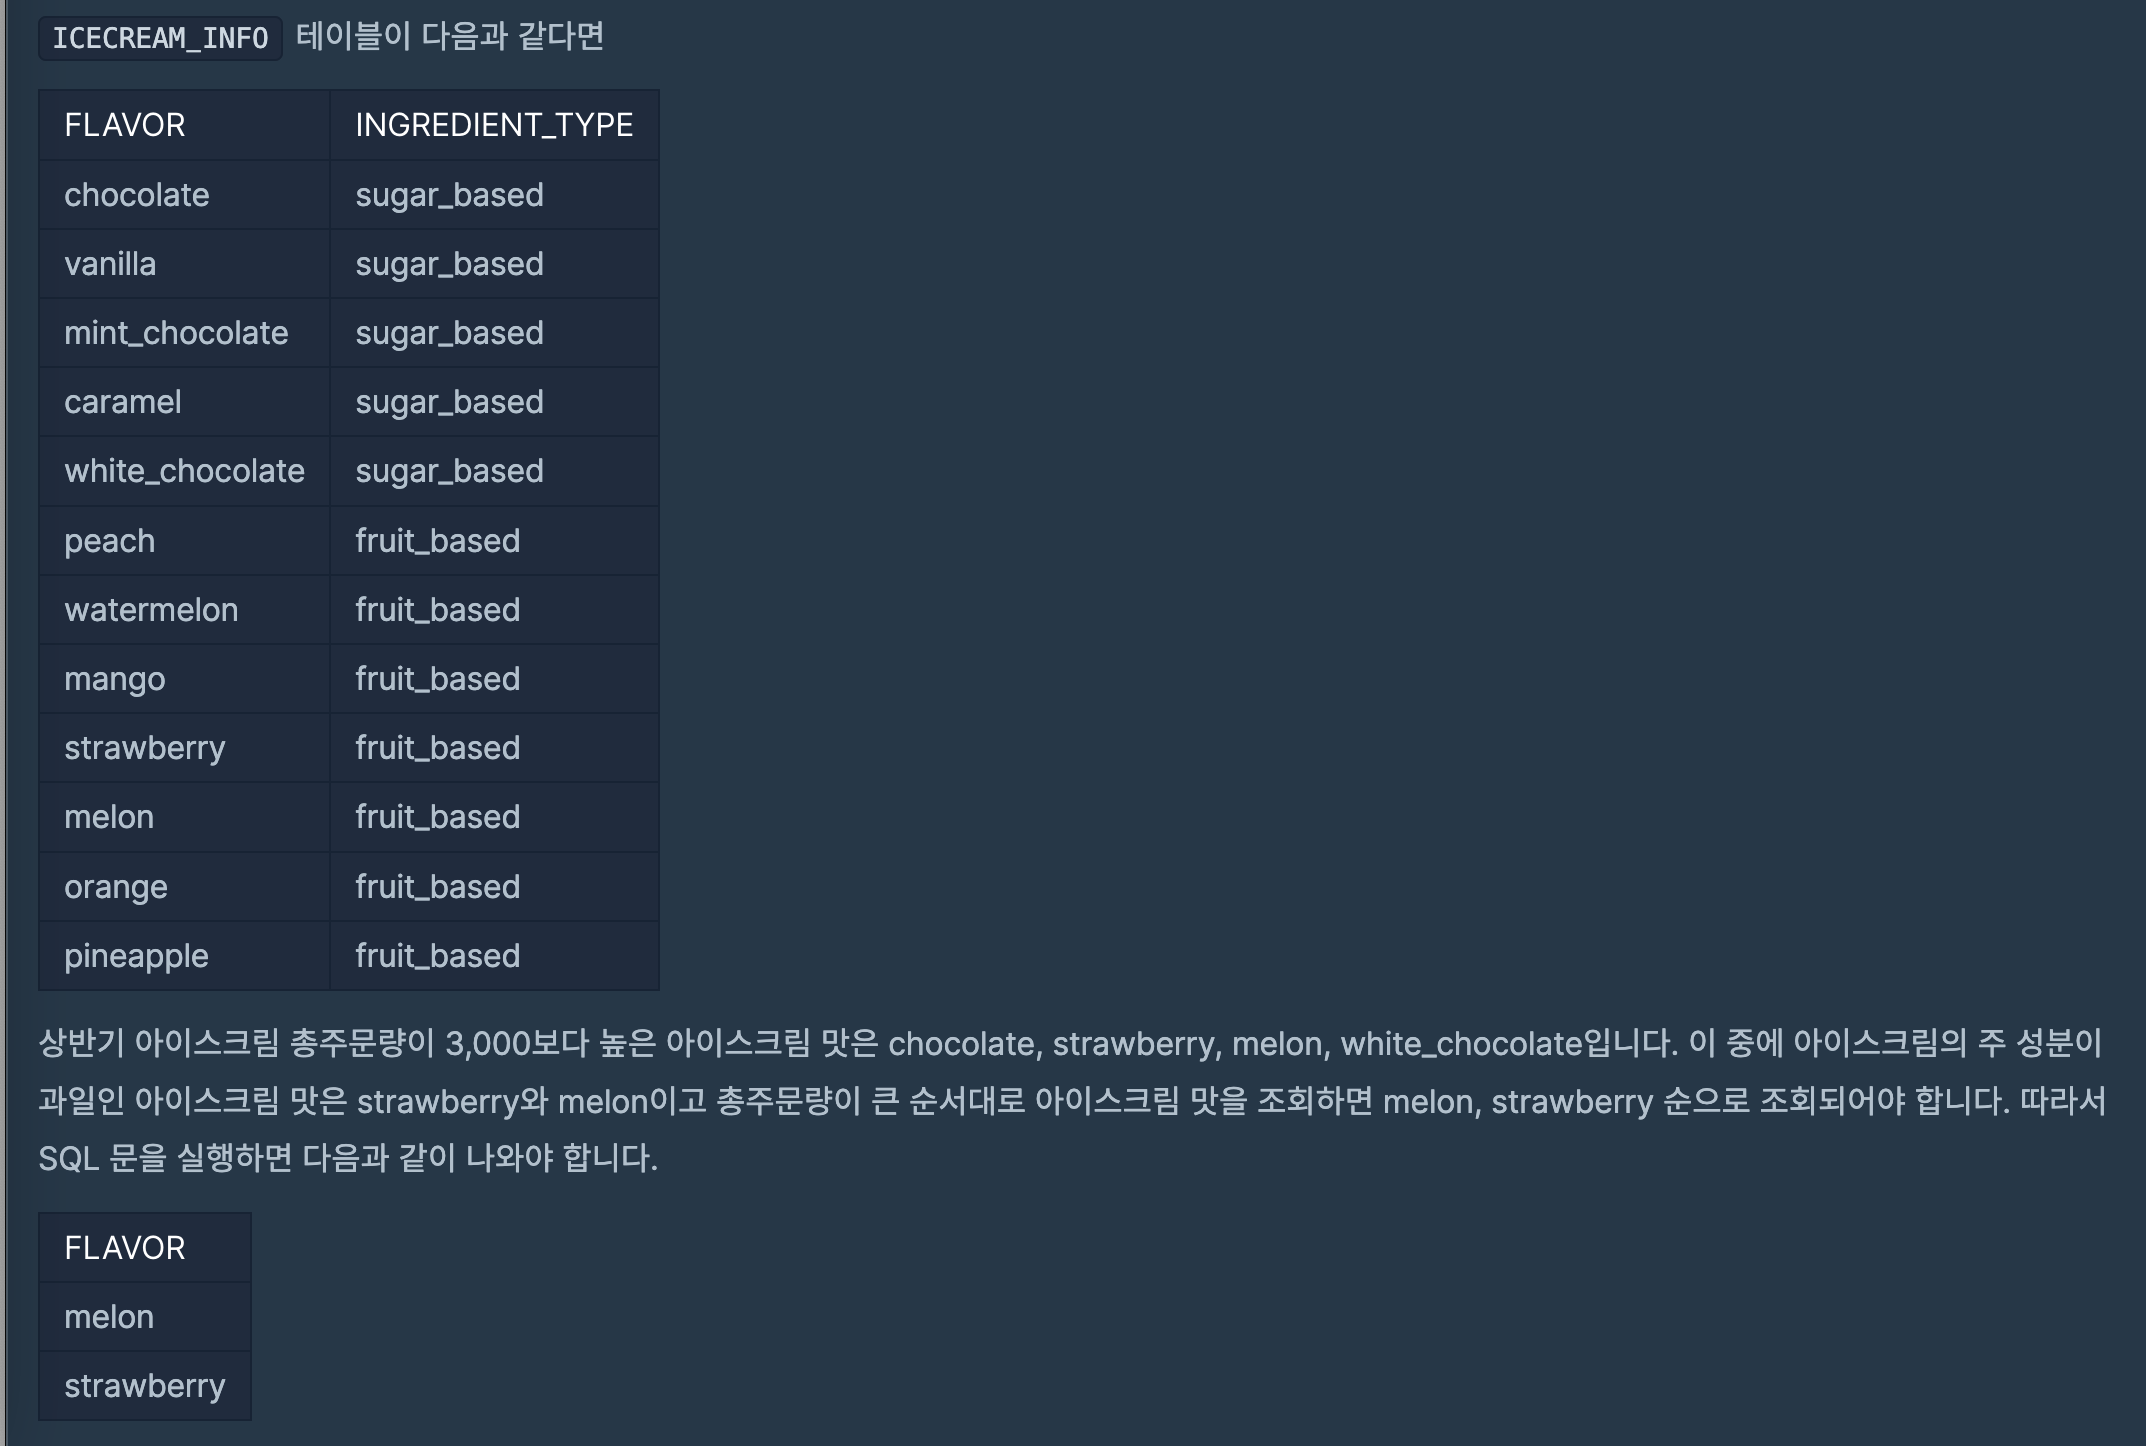
\includegraphics[width=100px]{../static/img/sql/p5-3.png}
\end{center}

\section*{풀이}
\label{sec:org430372a}

\section*{problem6: 평균 일일 대여 요금 구하기(level1)}
\label{sec:orga35d34d}
\begin{center}
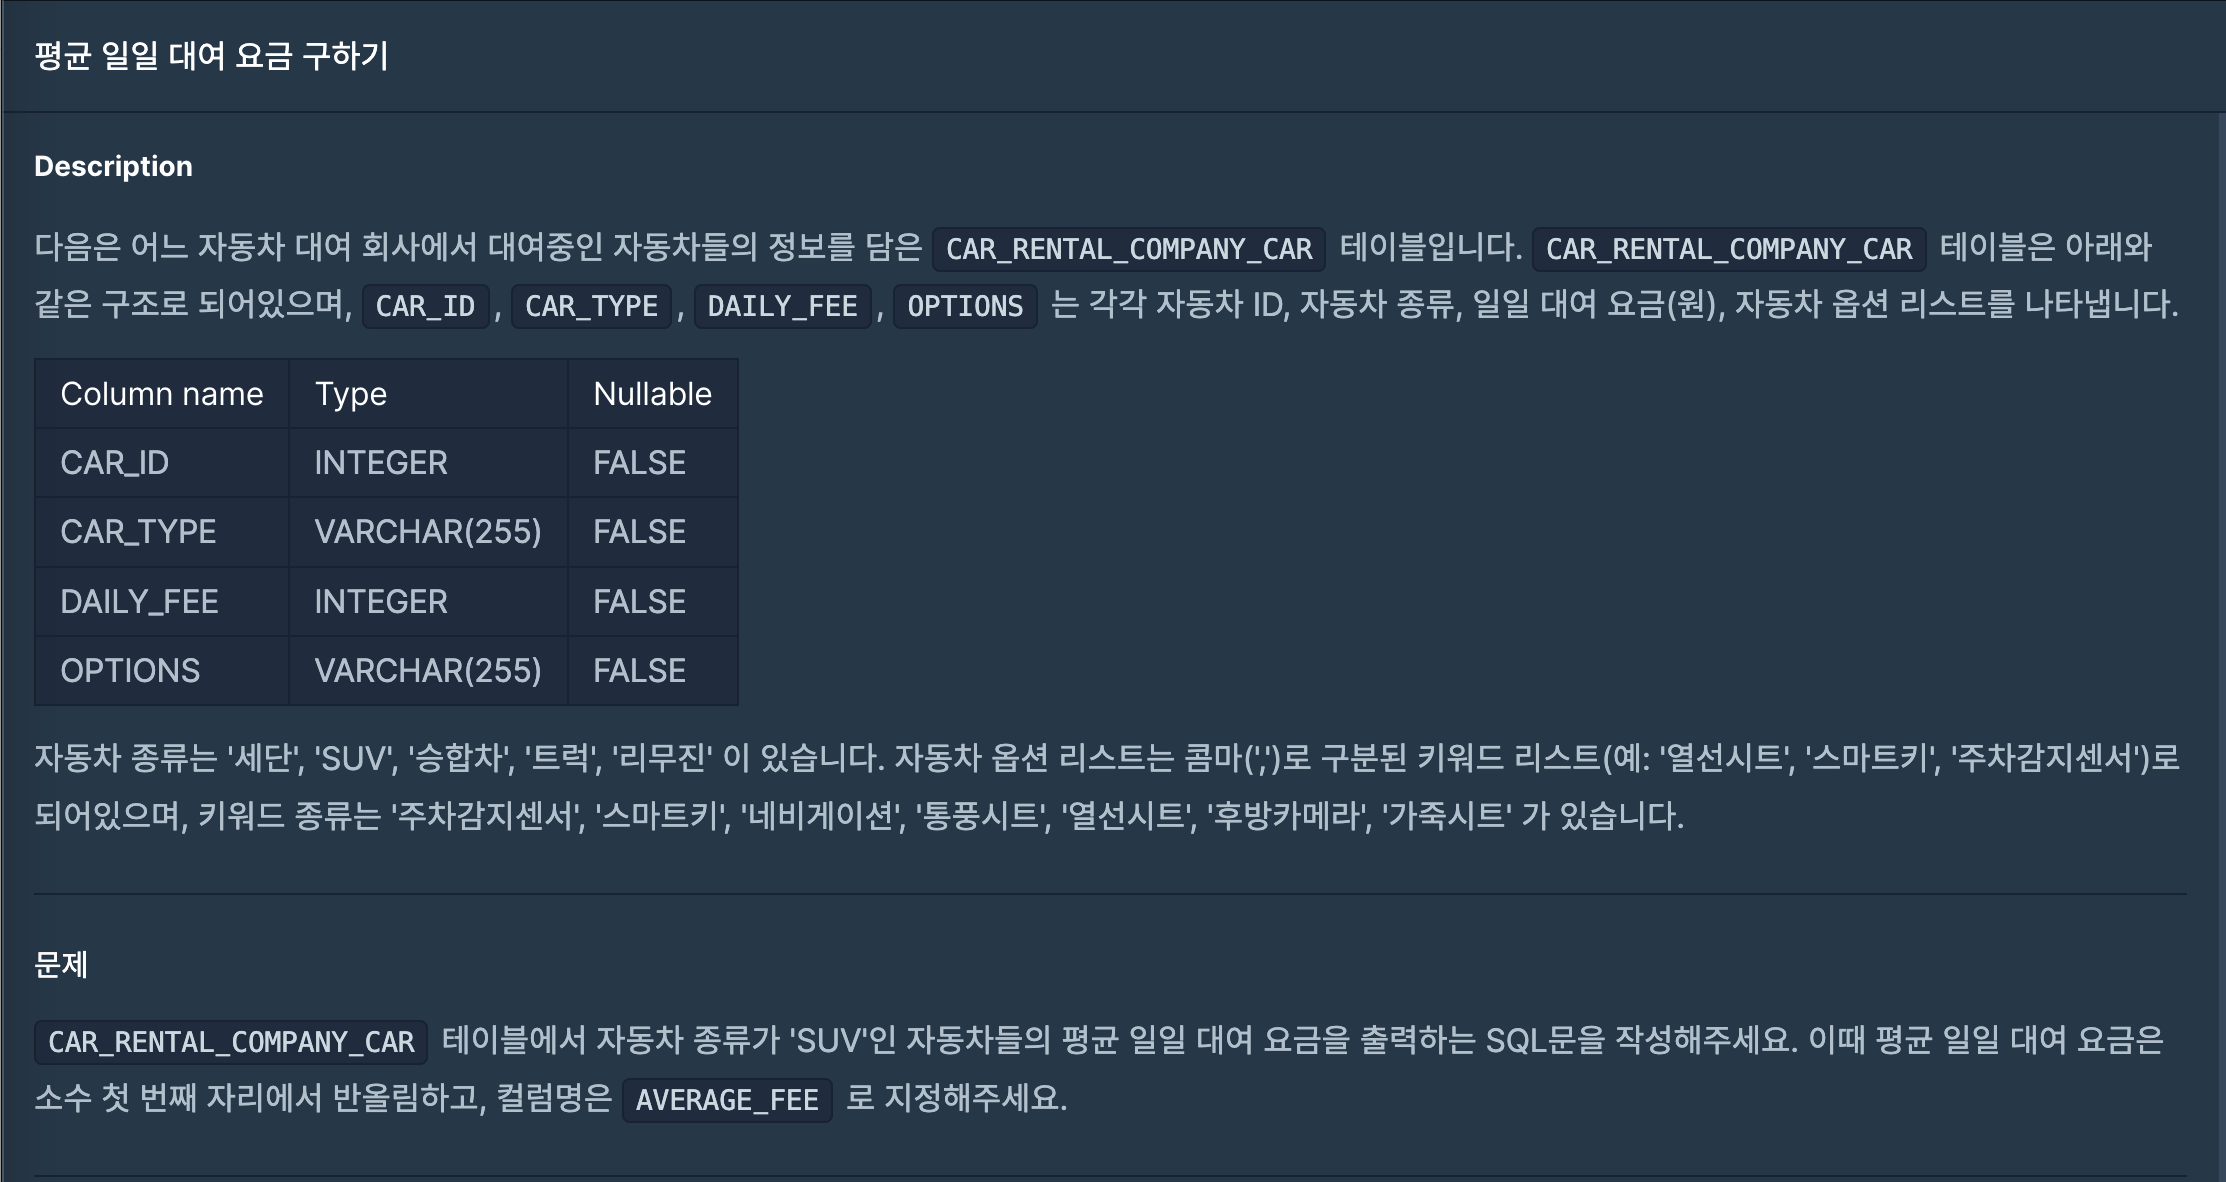
\includegraphics[width=100px]{../static/img/sql/p6-1.png}
\end{center}
\begin{center}
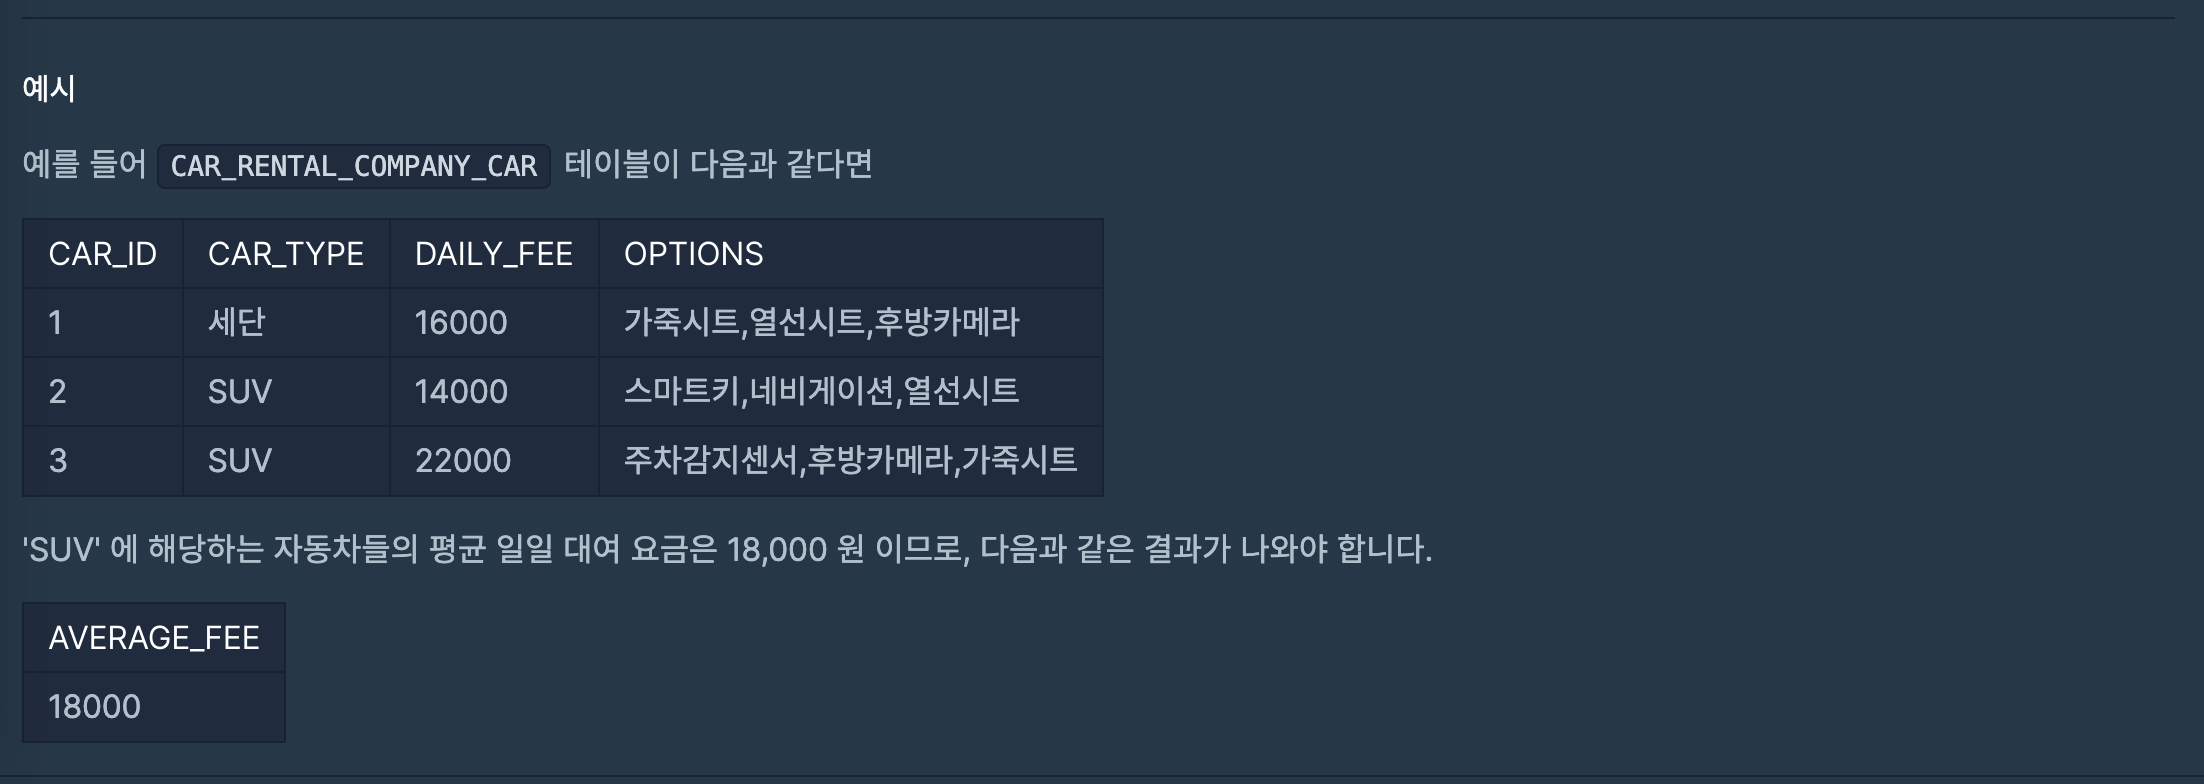
\includegraphics[width=100px]{../static/img/sql/p6-2.png}
\end{center}

\section*{풀이}
\label{sec:org6d1b71b}

\section*{problem7: 조건에 부합하는 중고거래 댓글 조회하기(level1)}
\label{sec:orgd2c4c08}
\begin{center}
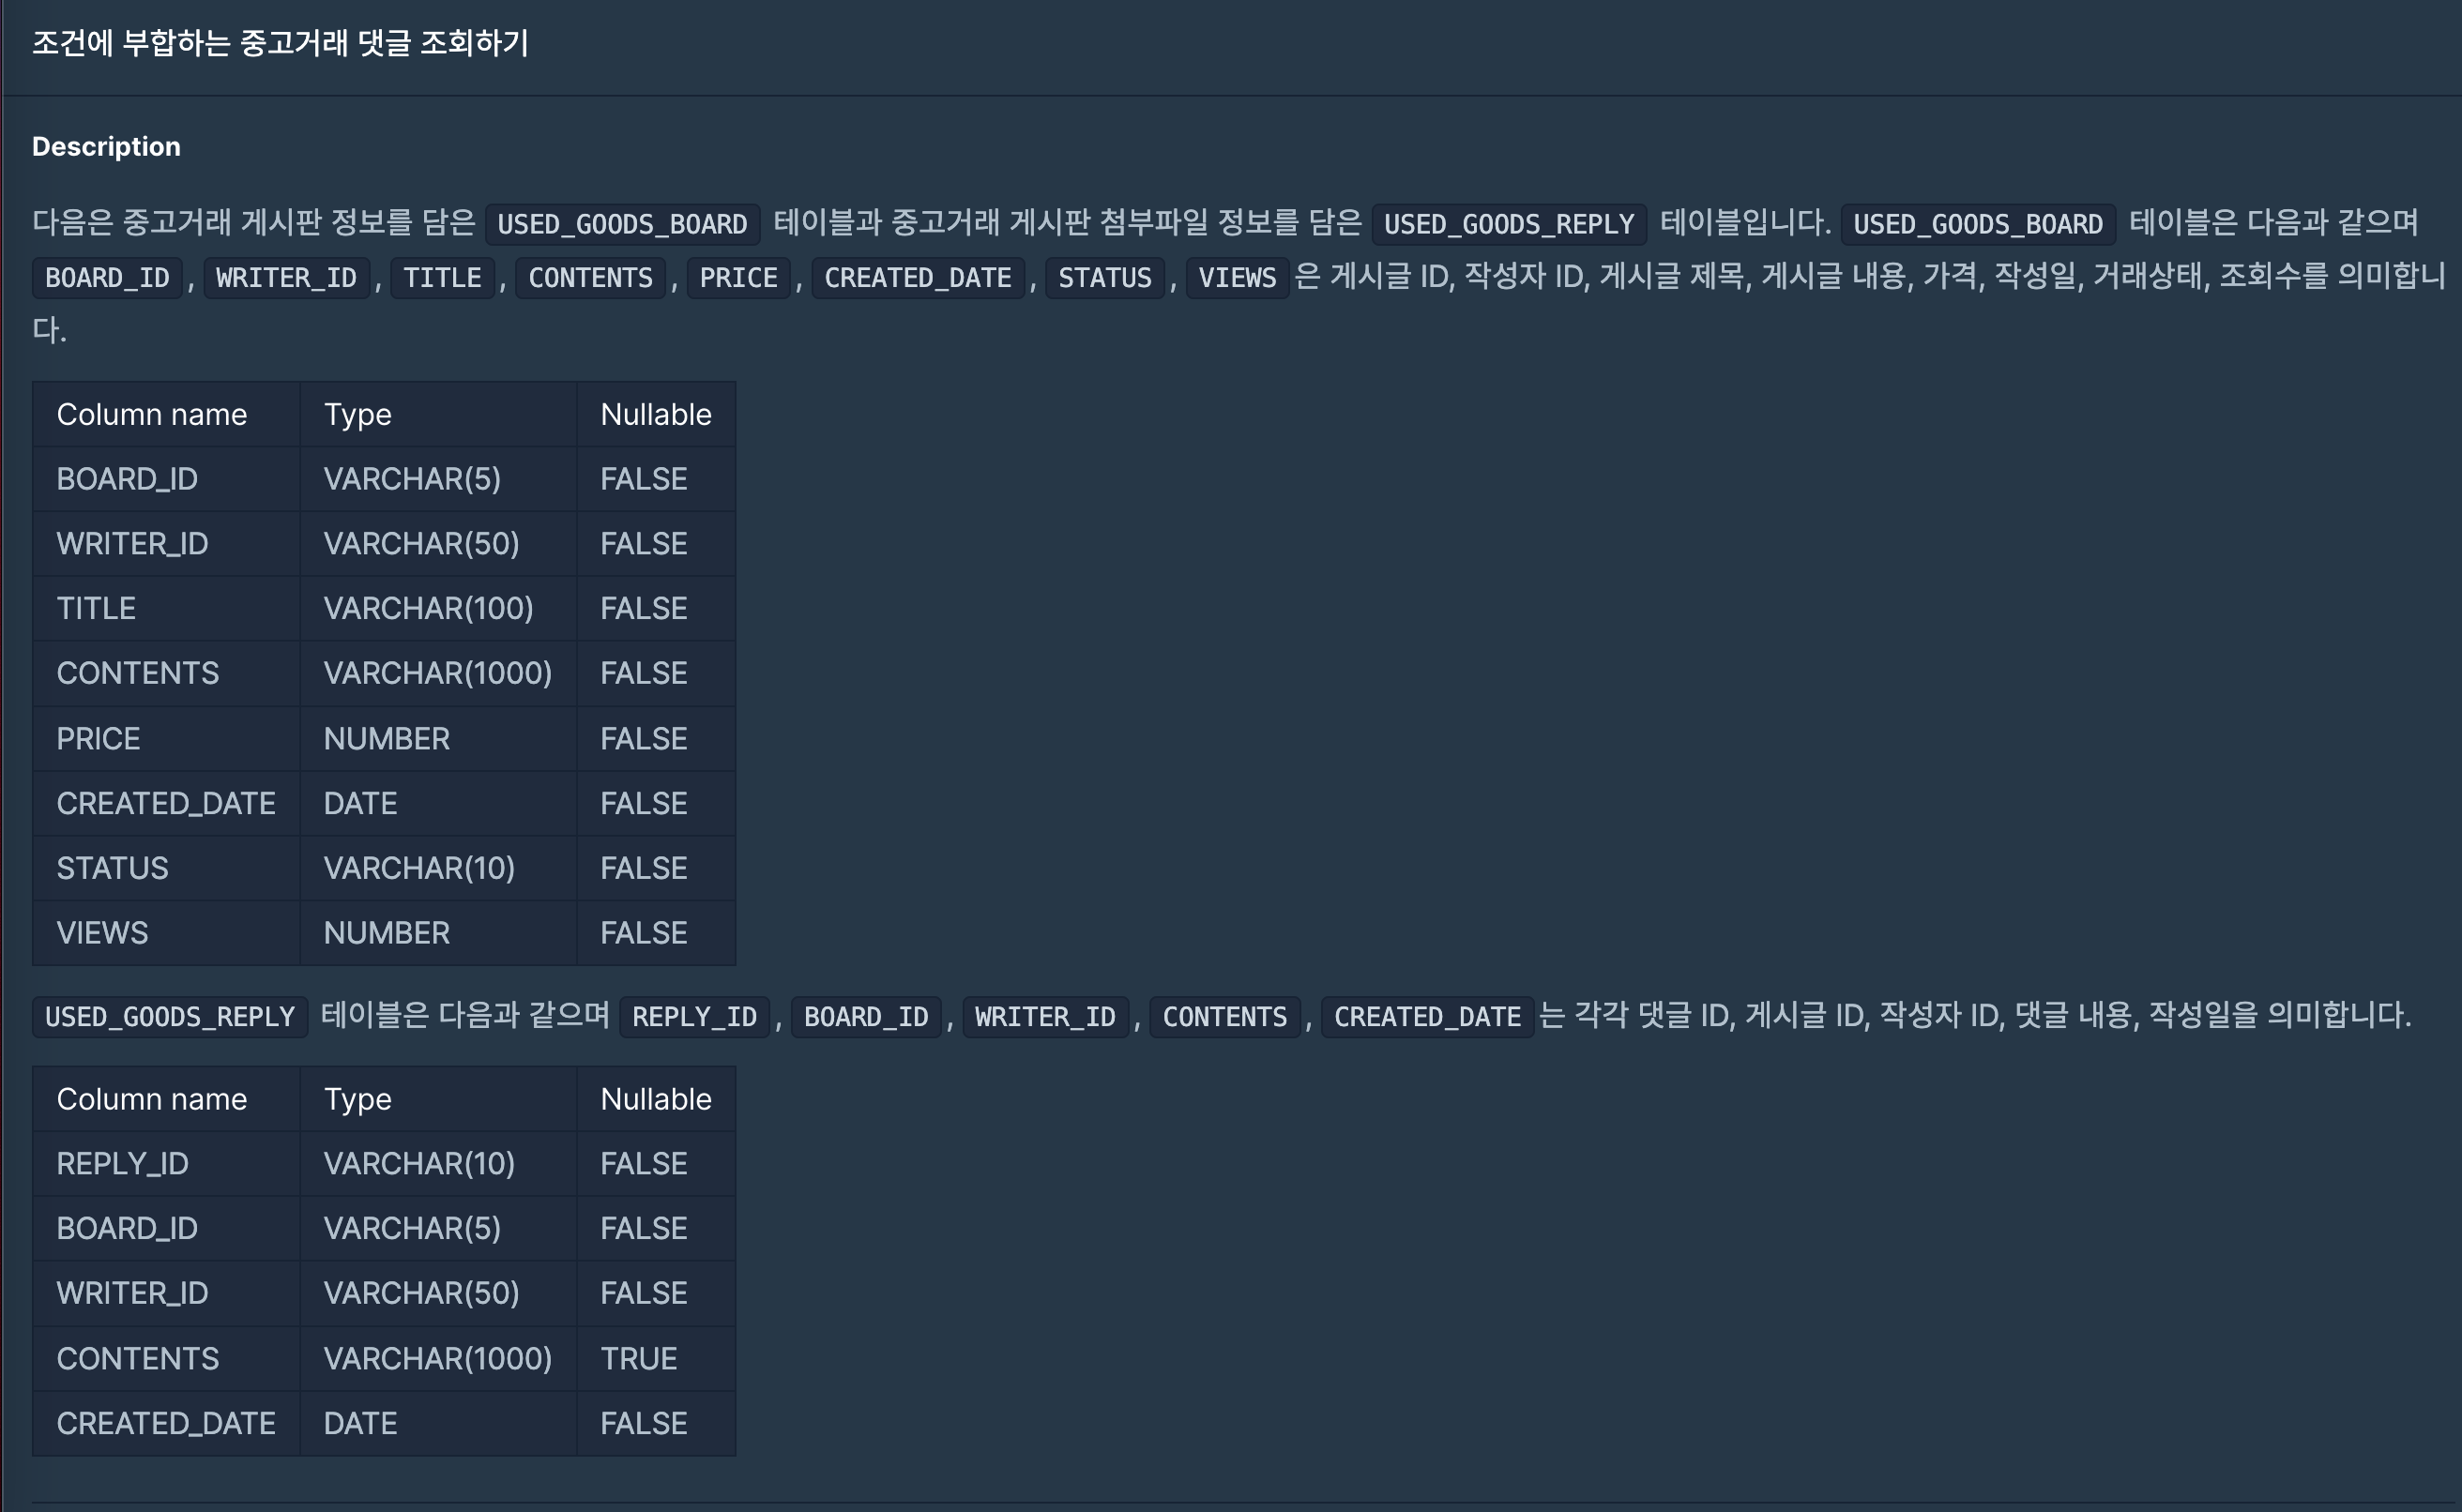
\includegraphics[width=100px]{../static/img/sql/p7-1.png}
\end{center}
\begin{center}
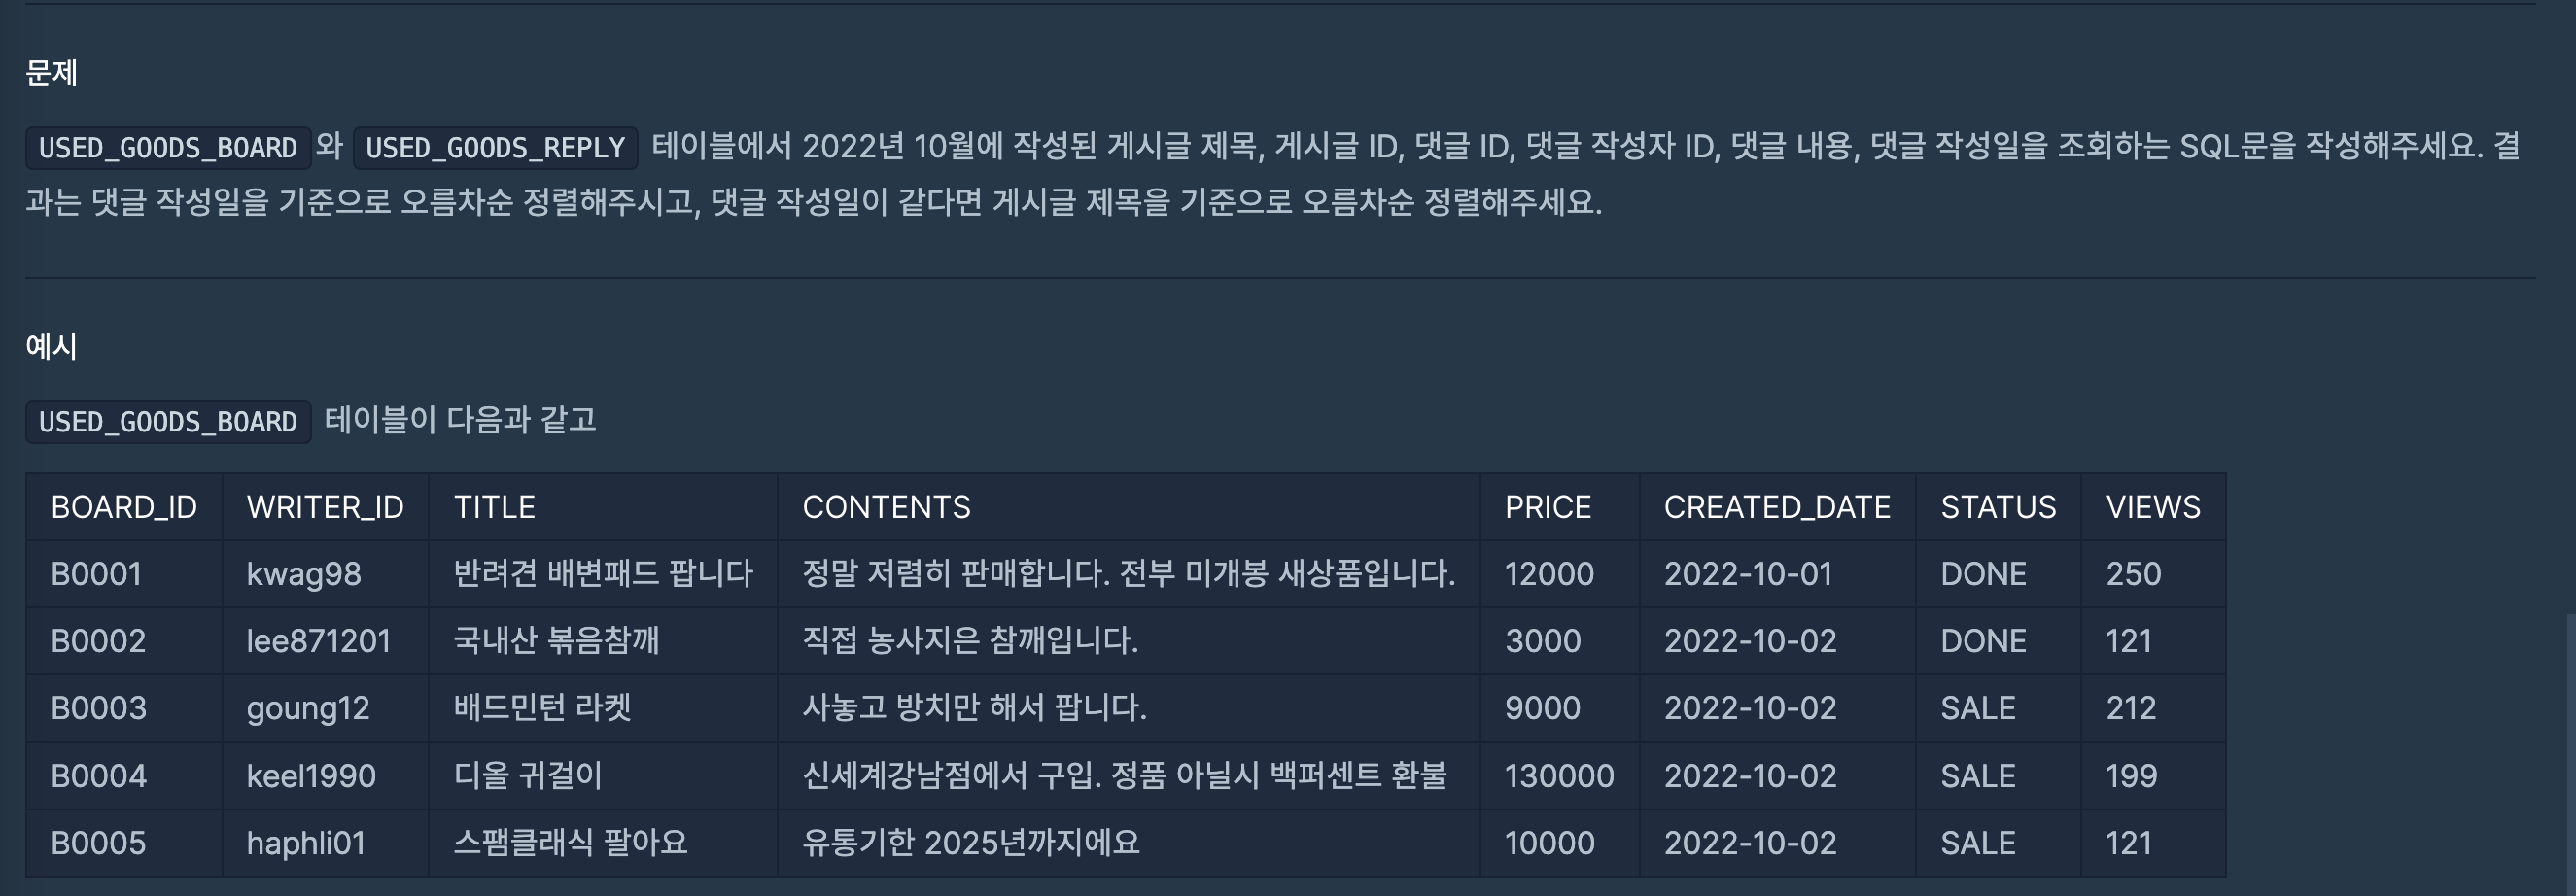
\includegraphics[width=100px]{../static/img/sql/p7-2.png}
\end{center}
\begin{center}
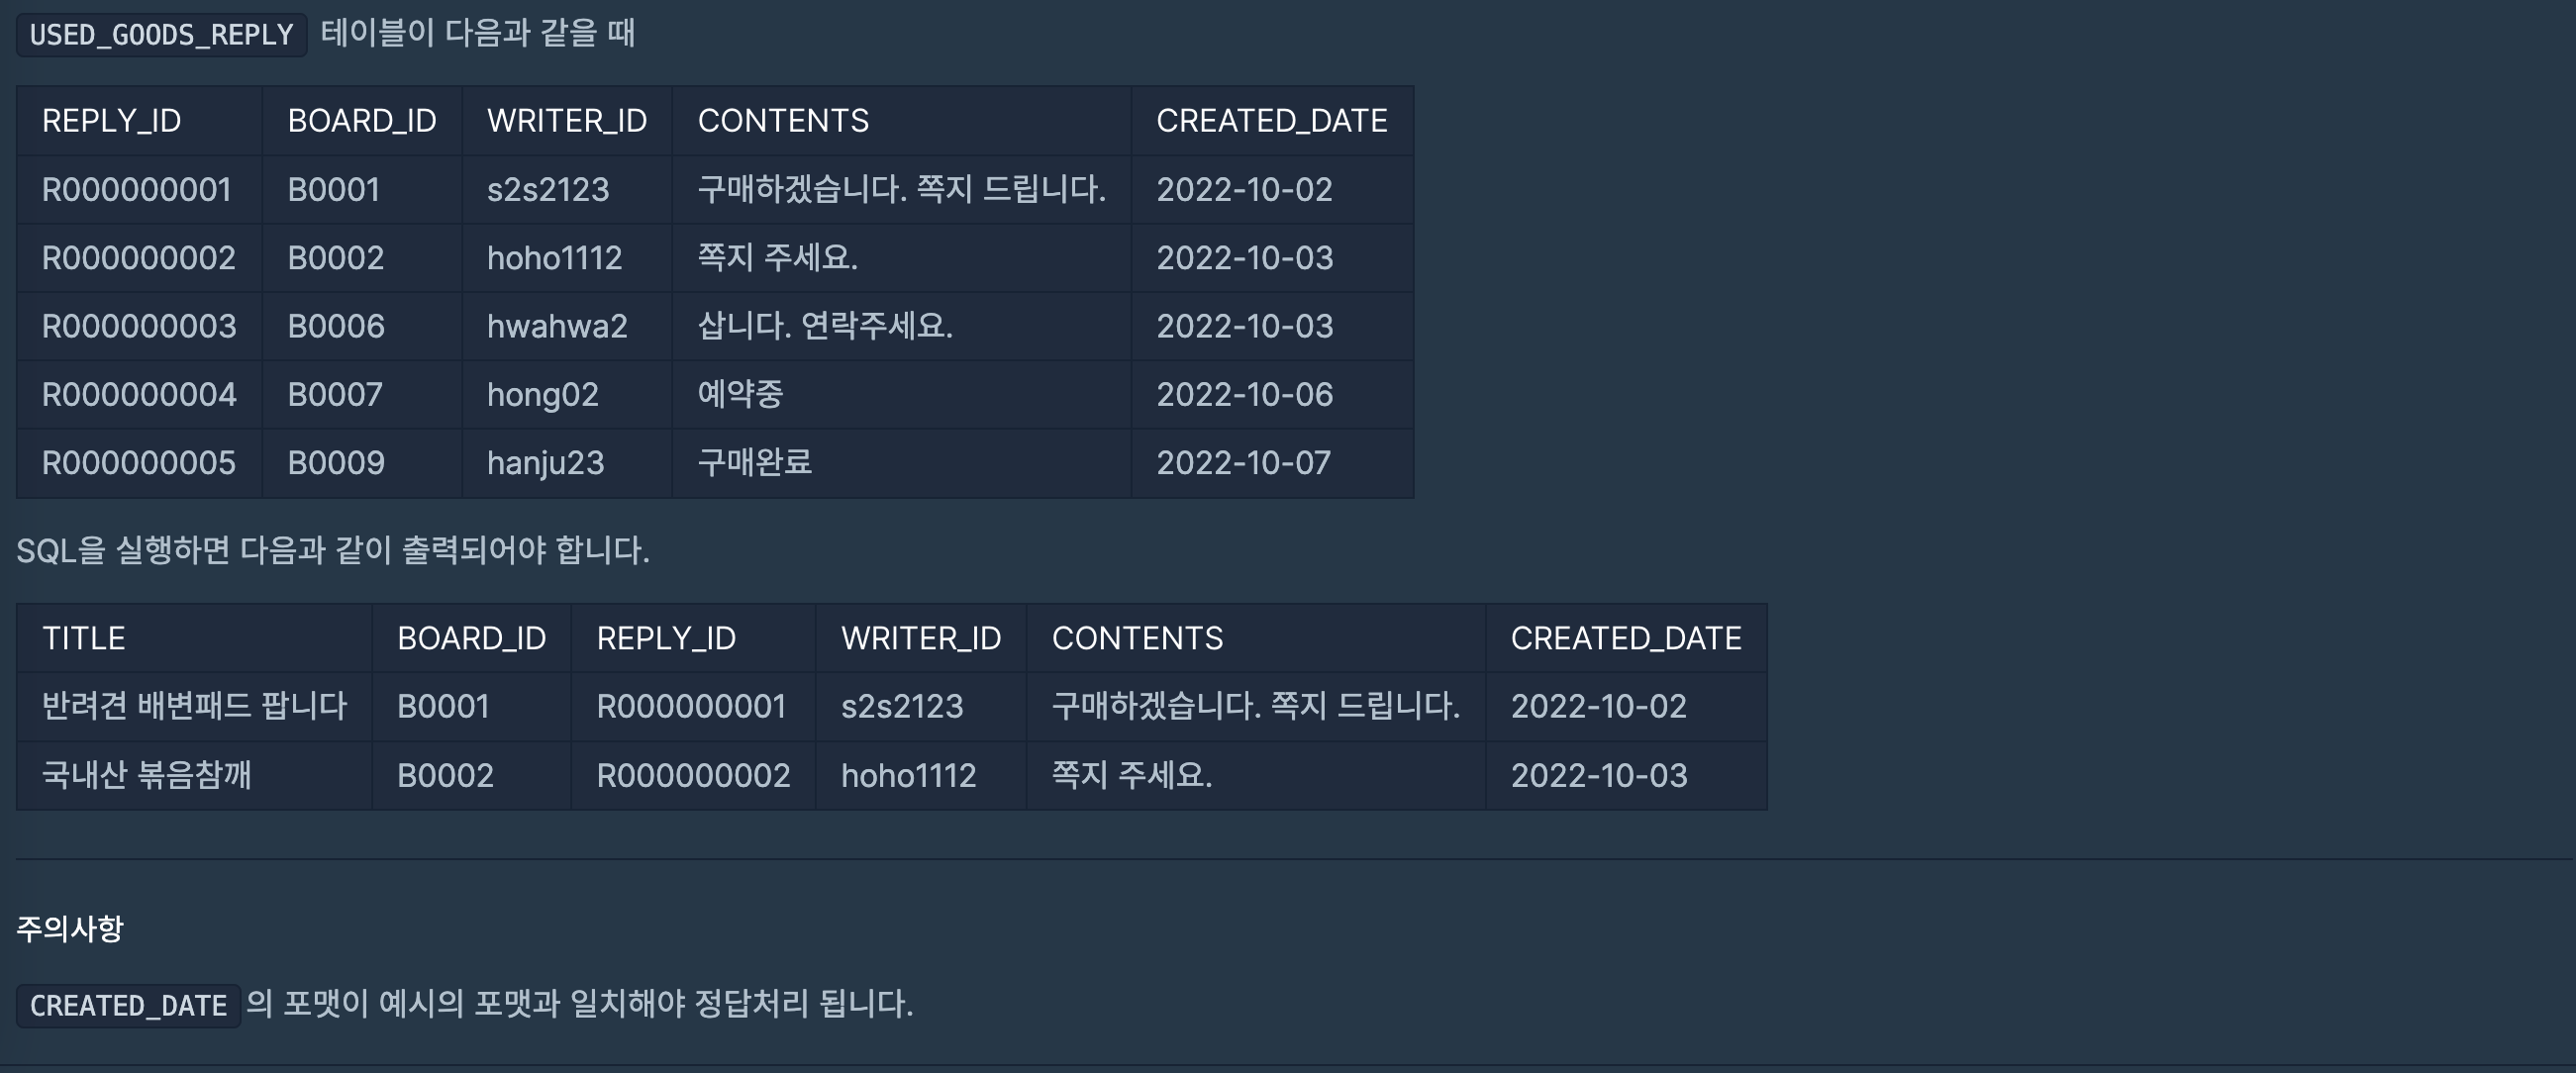
\includegraphics[width=100px]{../static/img/sql/p7-3.png}
\end{center}

\section*{풀이}
\label{sec:orgbffdccd}

\section*{problem8: 인기 있는 아이스크림(level1)}
\label{sec:orged1c410}
\begin{center}
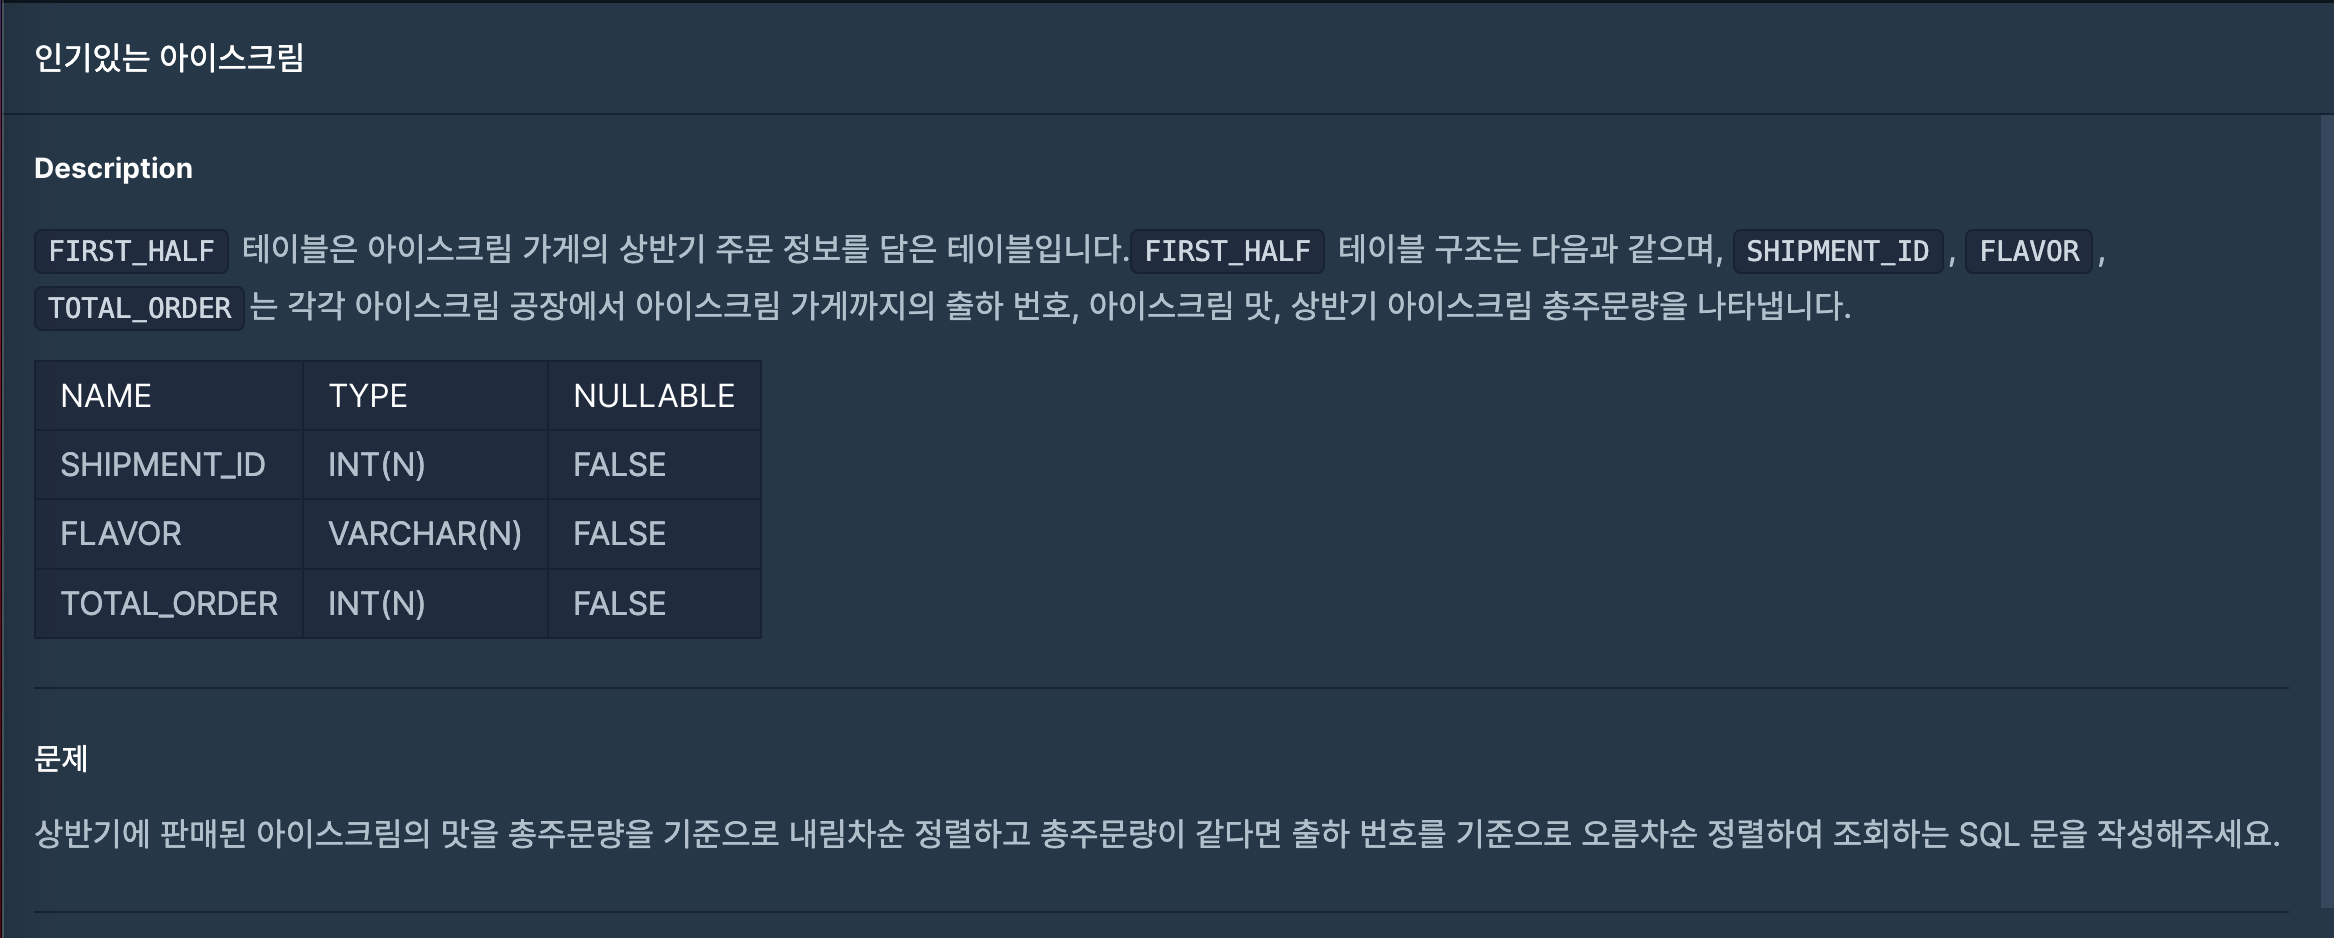
\includegraphics[width=100px]{../static/img/sql/p8-1.png}
\end{center}
\begin{center}
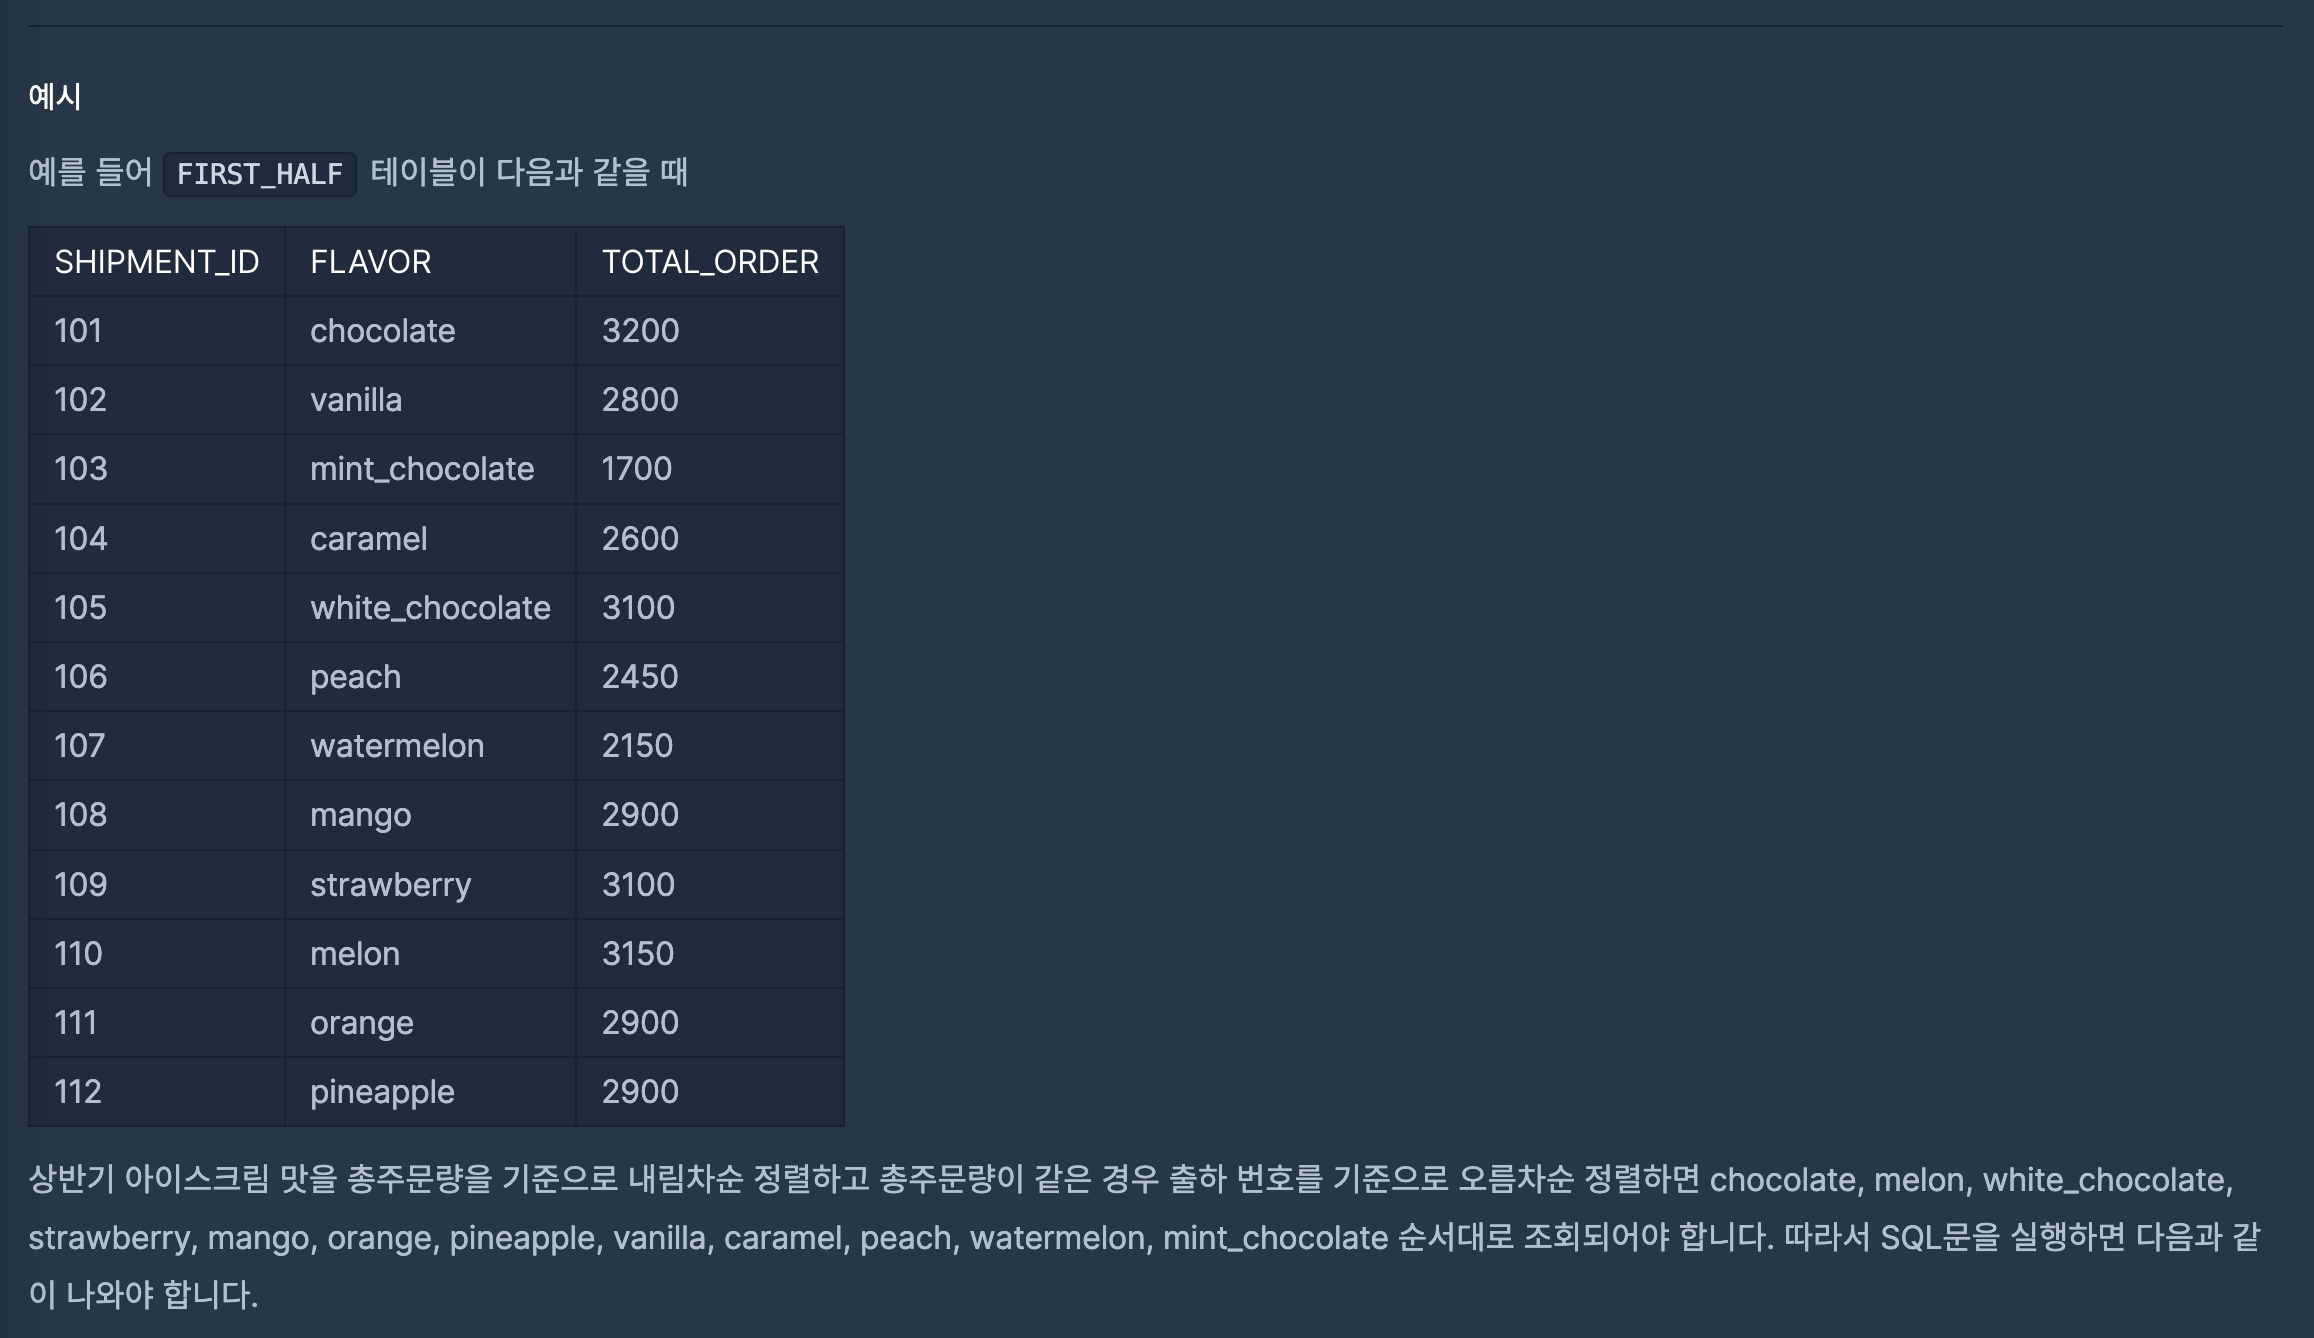
\includegraphics[width=100px]{../static/img/sql/p8-2.png}
\end{center}
\begin{center}
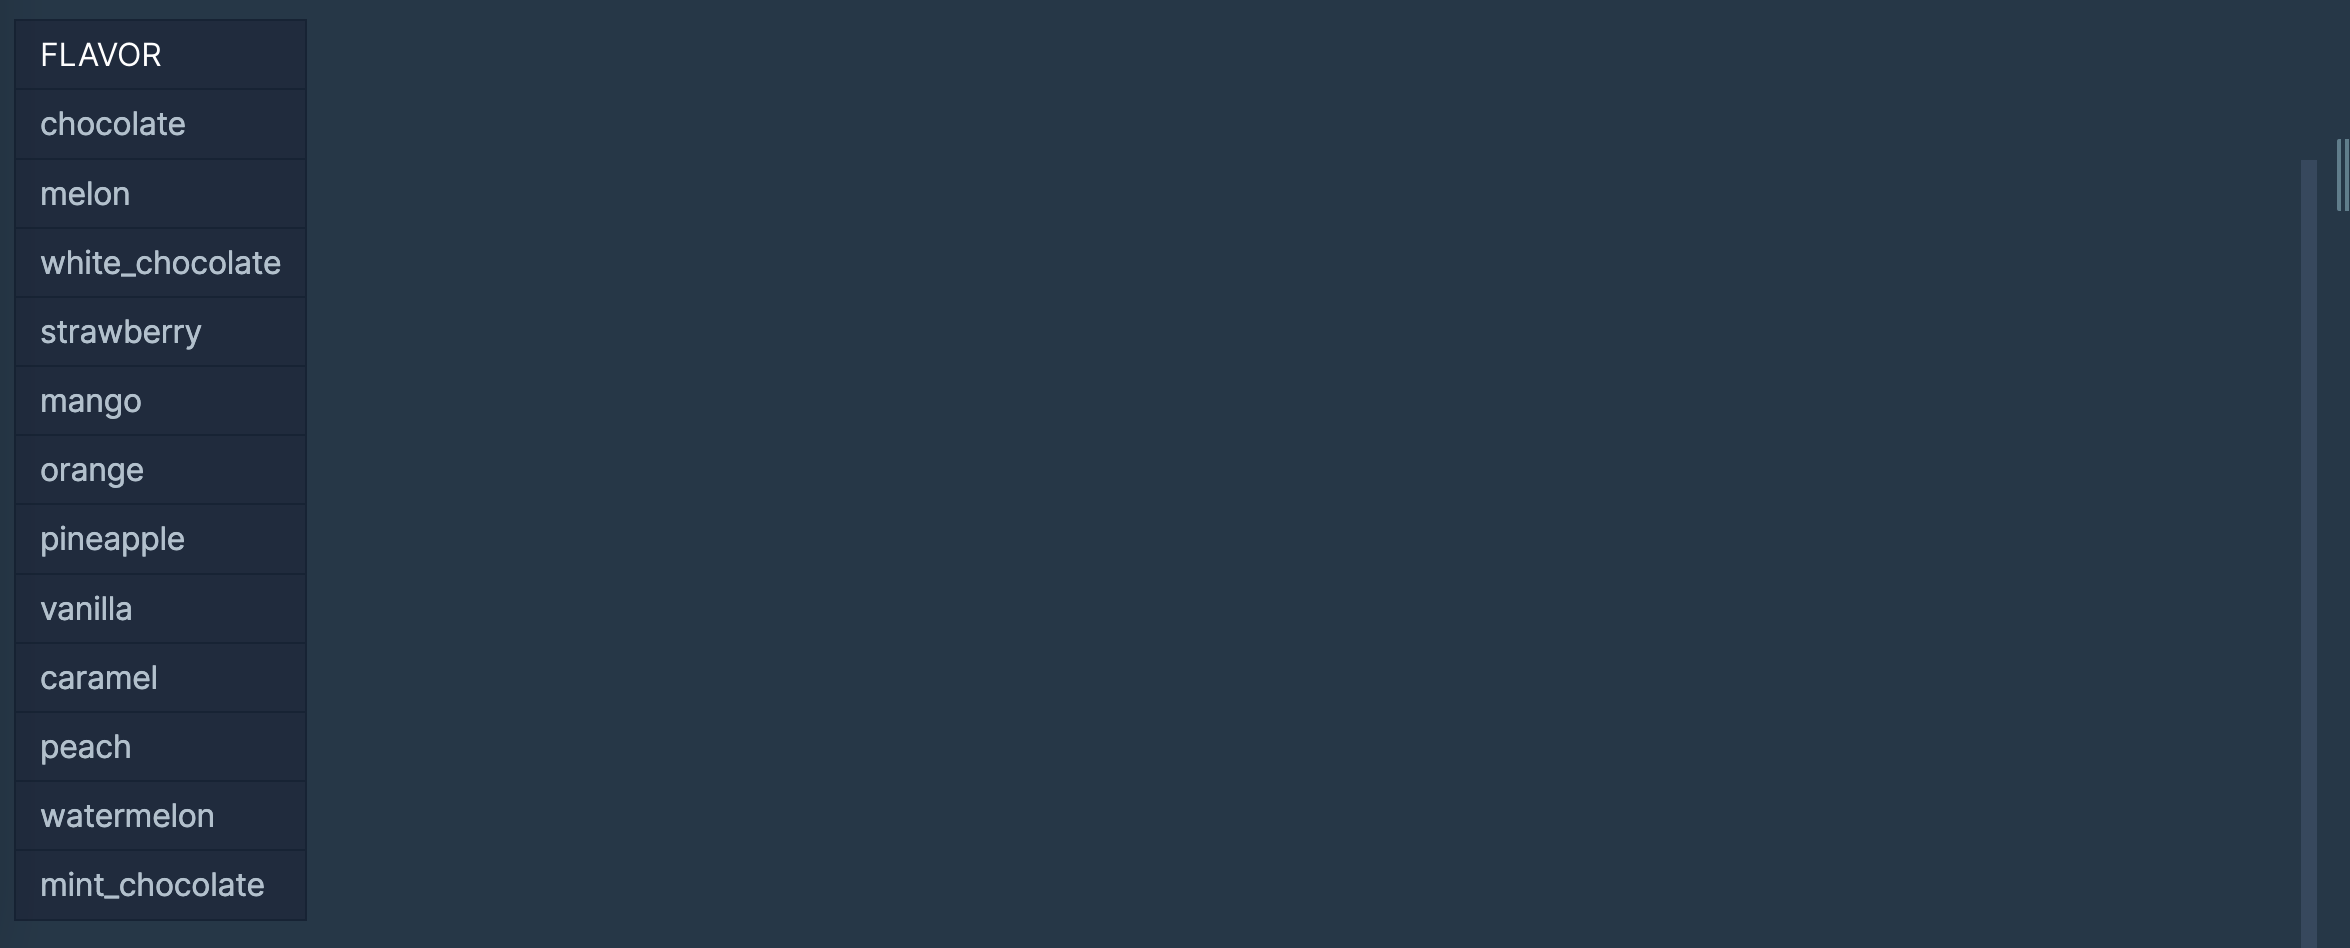
\includegraphics[width=100px]{../static/img/sql/p8-3.png}
\end{center}

\section*{풀이}
\label{sec:orgcacdc94}

\section*{problem9: 3월에 태어난 여성 회원 목록 출력하기(level2)}
\label{sec:org3257e52}
\begin{center}
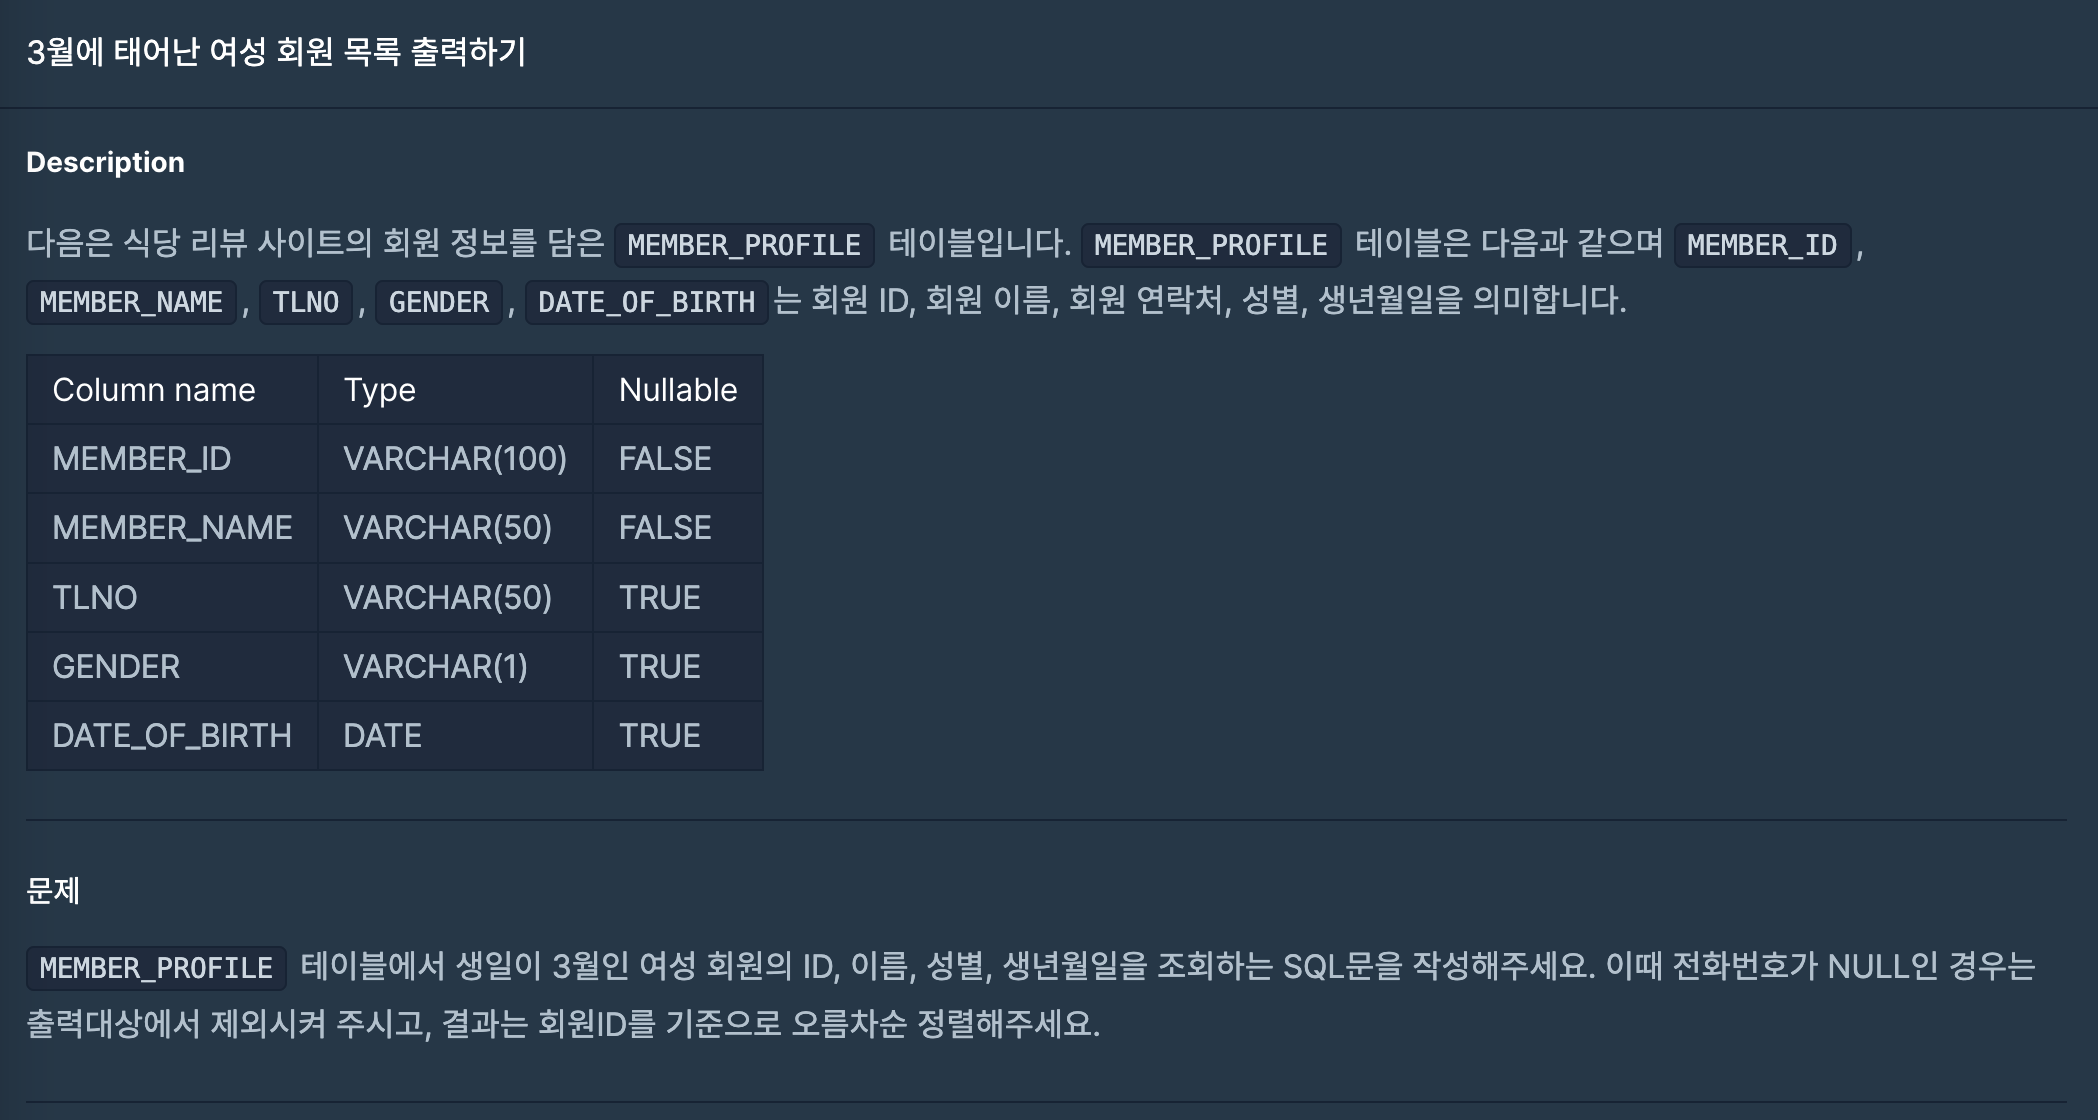
\includegraphics[width=100px]{../static/img/sql/p9-1.png}
\end{center}
\begin{center}
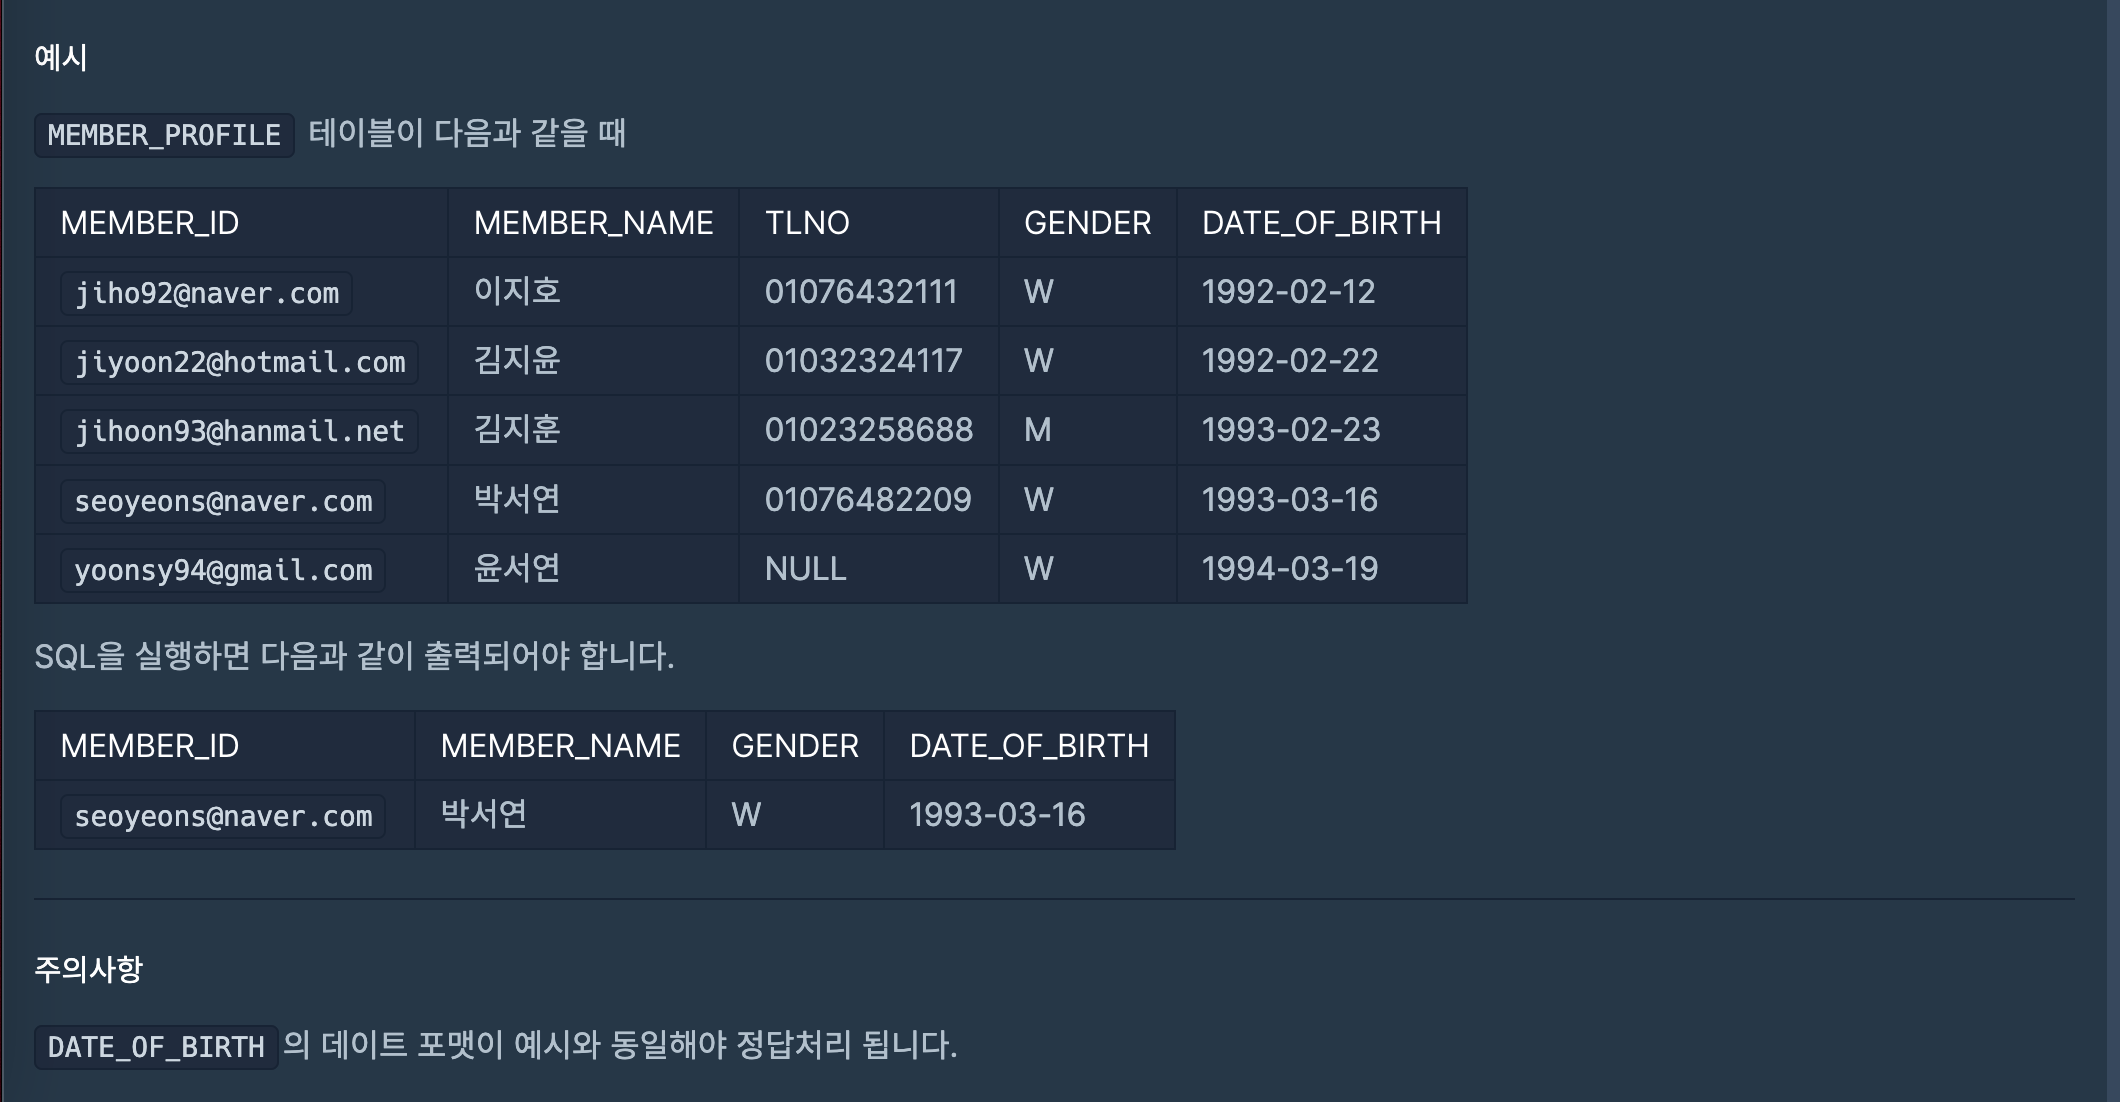
\includegraphics[width=100px]{../static/img/sql/p9-2.png}
\end{center}

\section*{풀이}
\label{sec:orgdf37db0}


\section*{problem10: 12세 이하인 여자환자 목록 출력하기(level1)}
\label{sec:org7cd0a7a}
\begin{center}
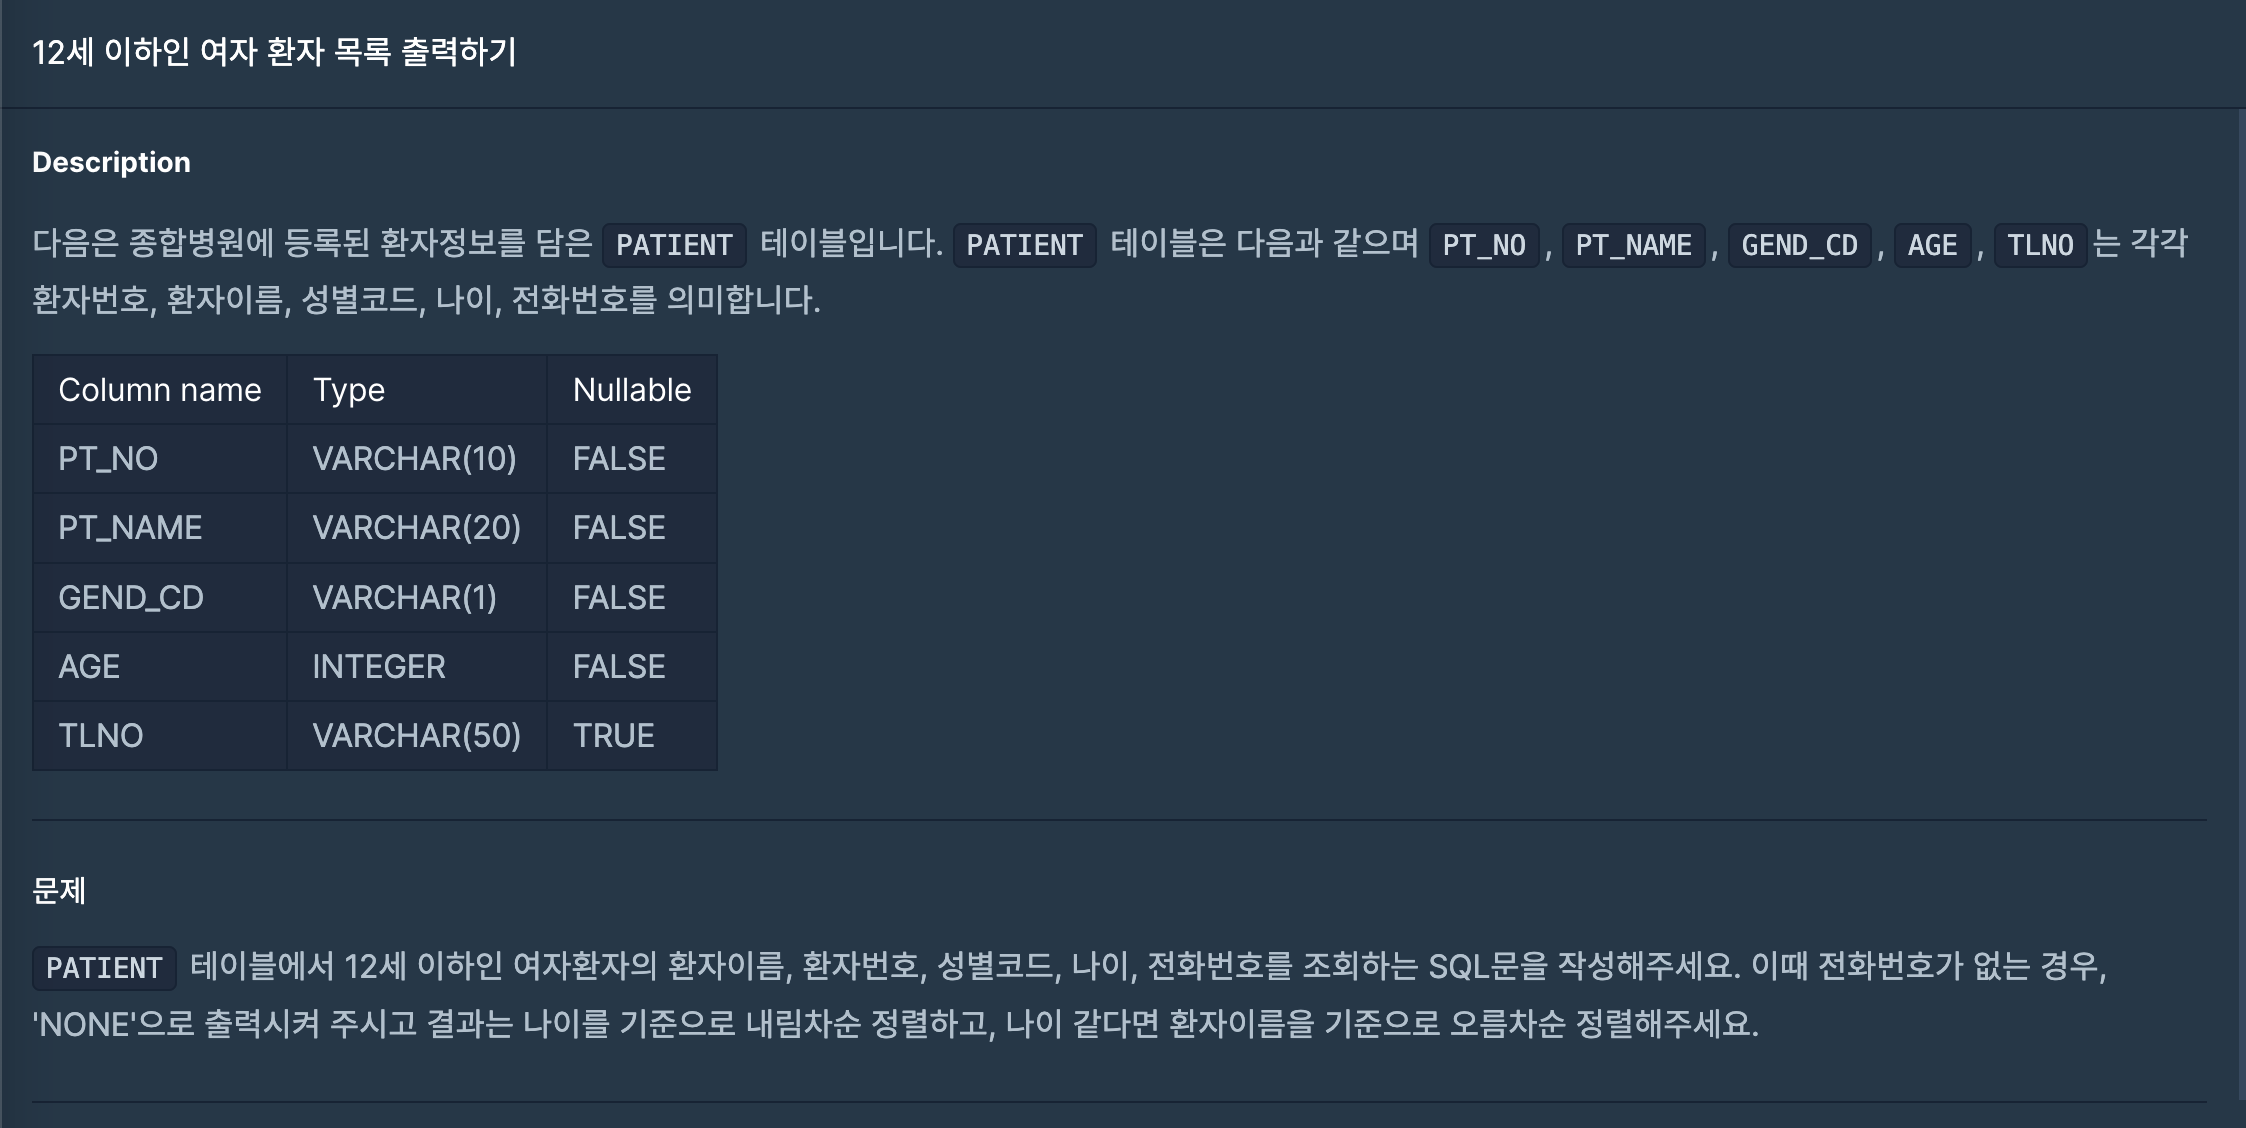
\includegraphics[width=100px]{../static/img/sql/p10-1.png}
\end{center}

\begin{center}
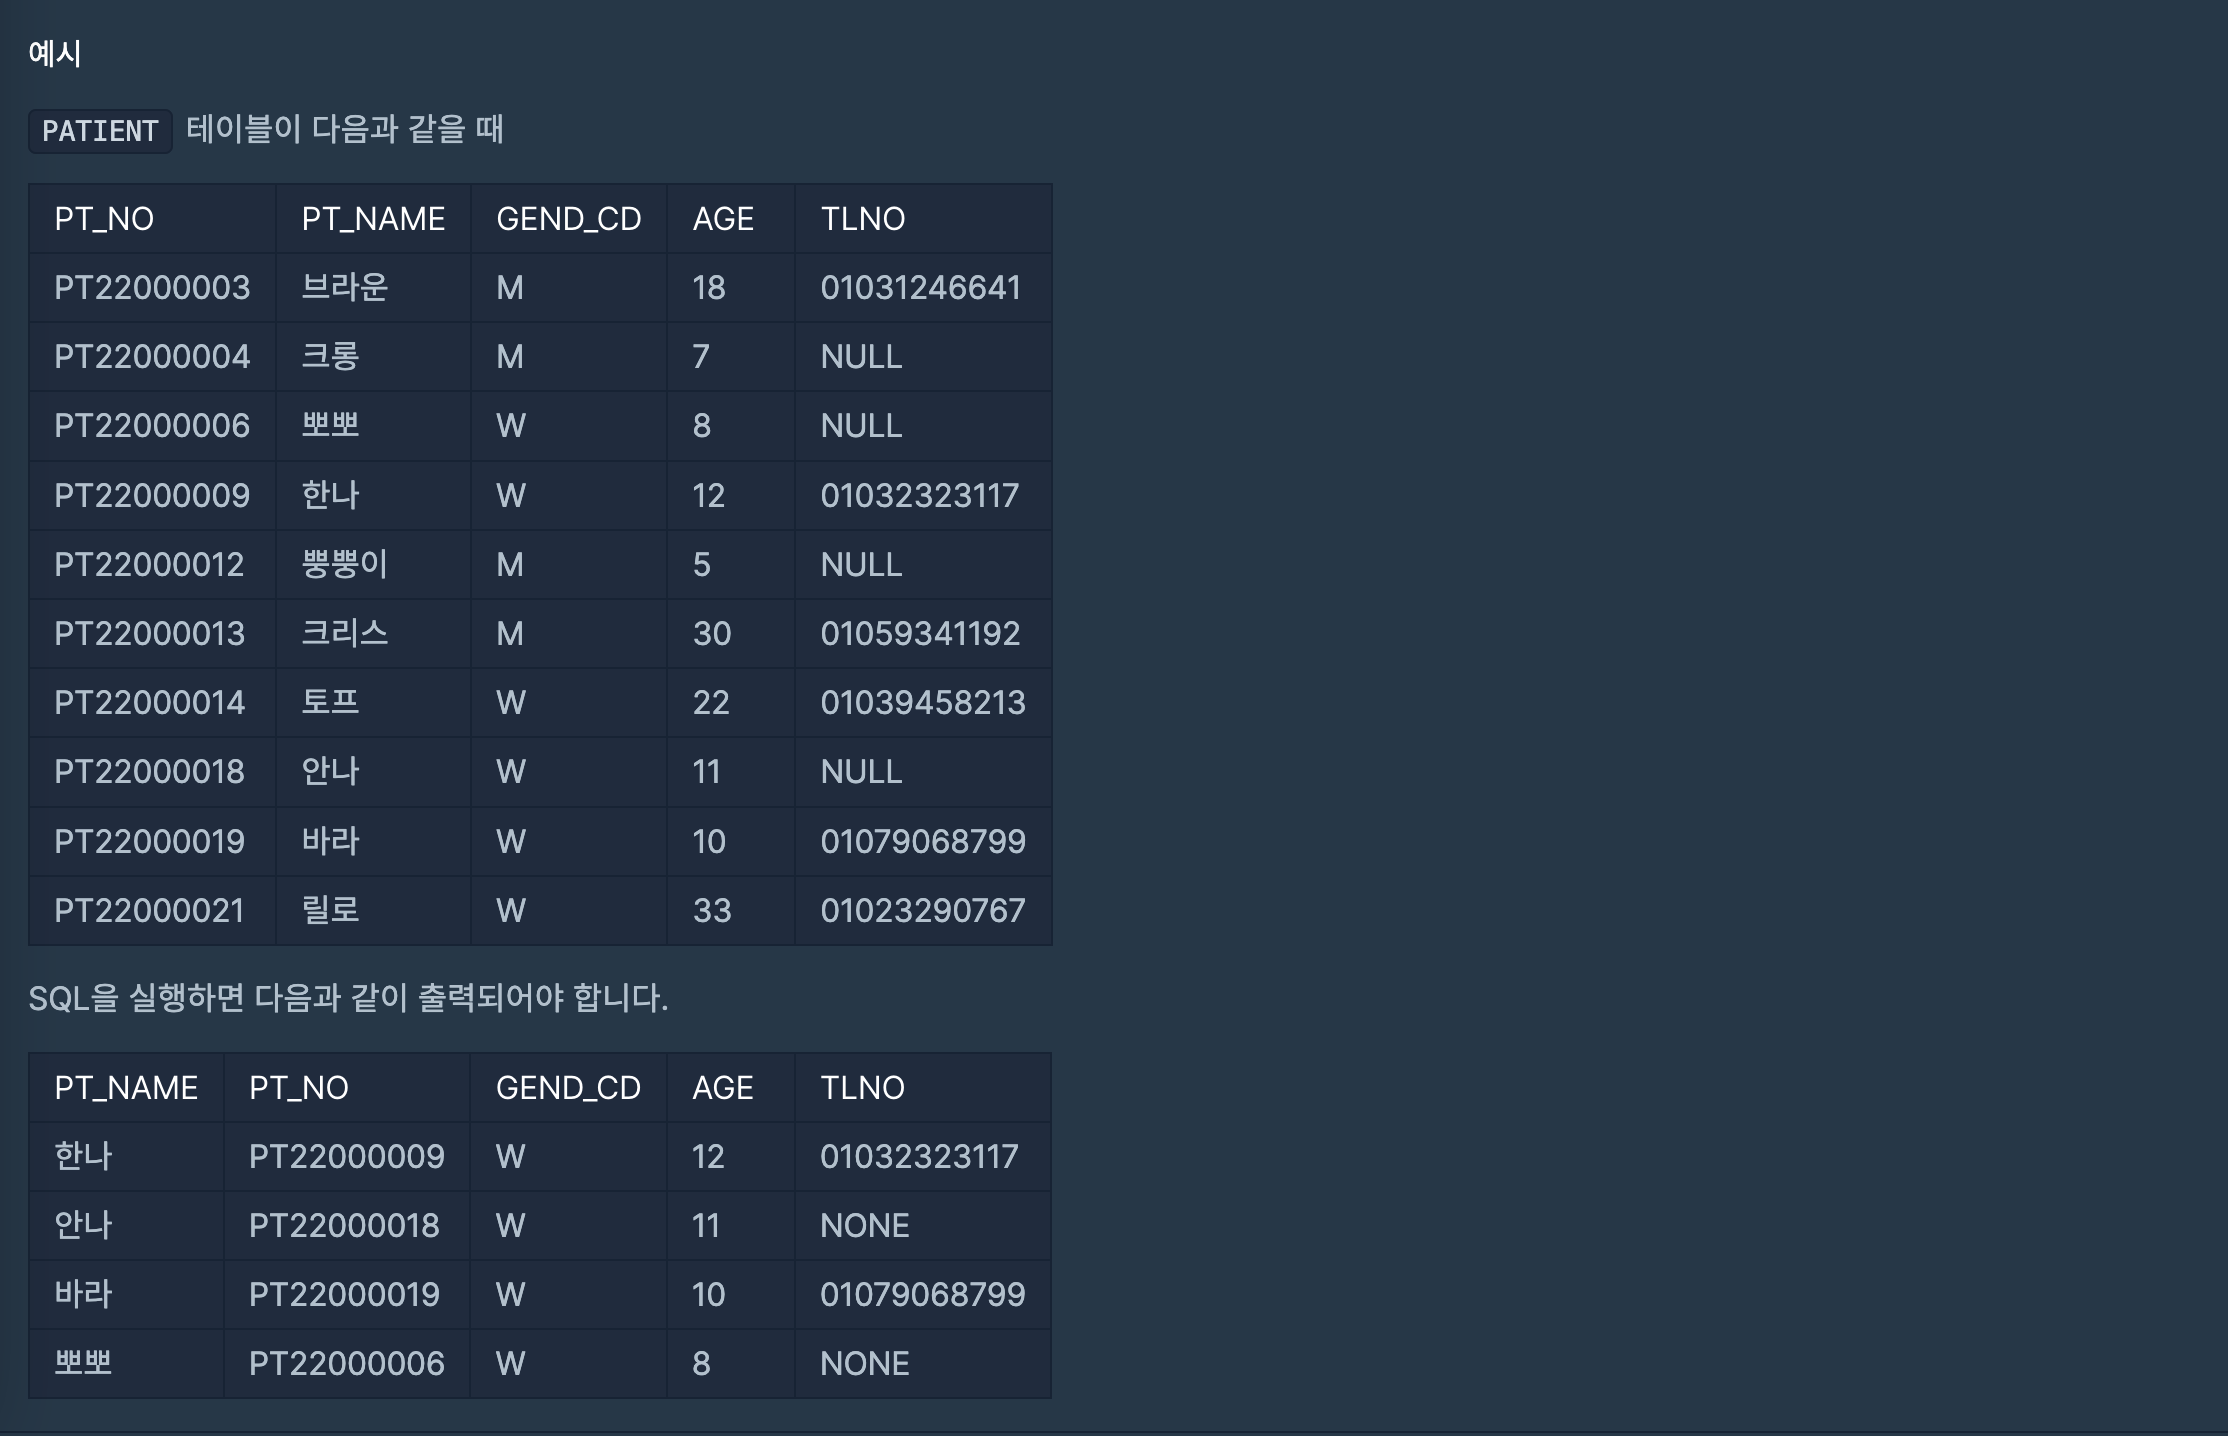
\includegraphics[width=100px]{../static/img/sql/p10-2.png}
\end{center}
\section*{풀이}
\label{sec:org60ebf7a}

\section*{problem11: 모든 레코드 조회하기(level1)}
\label{sec:org4be1dff}
\section*{풀이}
\label{sec:org0b831df}

\section*{problem12: 재구매가 일어난 상품과 회원 리스트 구하기(level2)}
\label{sec:orgfcace0b}
\section*{풀이}
\label{sec:orgb9235ce}

\section*{problem13: 역순 정렬하기(level1)}
\label{sec:orgcc2d5b7}
\section*{풀이}
\label{sec:org050f148}

\section*{problem14: 오프라인/온라인 판매 데이터 통합하기(level4)}
\label{sec:orgec782b1}
\section*{풀이}
\label{sec:orga08779d}

\section*{problem15: 아픈 동물 찾기(level1)}
\label{sec:org026def9}
\section*{풀이}
\label{sec:org91b5bfe}

\section*{problem16: 어린 동물 찾기(level1)}
\label{sec:org8bc9132}
\section*{풀이}
\label{sec:org6cfc858}

\section*{problem17: 동물의 아이디와 이름(level1)}
\label{sec:org5c0ddf8}
\section*{풀이}
\label{sec:org789fe85}

\section*{problem18: 여러기준으로 정렬하기(level1)}
\label{sec:org6428a00}
\section*{풀이}
\label{sec:org0e2c5d3}

\section*{problem19: 상위 n개 레코드(level1)}
\label{sec:org8187e21}
\section*{풀이}
\label{sec:org99a6d70}

\section*{problem20: 조건에 맞는 회원수 구하기(level1)}
\label{sec:org18b4e3c}
\section*{풀이}
\label{sec:orgf7050fa}
\end{document}